\documentclass[fr]{../../../eplsummary}

\usepackage{../../../eplunits}
\usepackage{../../../eplelec}
\usepackage{circuitikz}
\sisetup{detect-all}
\usepackage[makeroom]{cancel}
\usepackage{amsmath,mathtools}
\usepackage{multicol}
\usepackage{float}
\usepackage{trimclip}


\newcommand{\Ueff}{U_\text{eff}}
\newcommand{\Ieff}{I_\text{eff}}
\newcommand{\Umr}{U_\text{moy,r}}
\newcommand{\Imr}{I_\text{moy,r}}
\newcommand{\Up}{\bar{U}}
\newcommand{\Ip}{\bar{I}}
\newcommand{\Zp}{\bar{Z}}
\newcommand{\Icc}{I_\text{cc}}
\newcommand\numberthis{\addtocounter{equation}{1}\tag{\theequation}}

\makeatletter
\providecommand\add@text{}
\renewcommand\u[1]{%
  \gdef\add@text{[\si{#1}\gdef\add@text{}]}}% 
\renewcommand\tagform@[1]{%
  \maketag@@@{\llap{\add@text\quad}(\ignorespaces#1\unskip\@@italiccorr)}%
}
\newenvironment{Figure}
  {\par\medskip\noindent\minipage{\linewidth}}
  {\endminipage\par\medskip}

\usepackage{tikz}
\usetikzlibrary{arrows,shapes,positioning,shadows,trees}


\tikzset{
  basic/.style  = {draw, text width=6cm, drop shadow, font=\sffamily, rectangle},
  root/.style   = {basic, rounded corners=2pt, thin, align=center,
                   fill=green!30},
  level 2/.style = {basic, rounded corners=6pt, thin,align=center, fill=green!60,
                   text width=12em},
  level 3/.style = {basic, thin, align=left, fill=pink!60, text width=8em}
}

\hypertitle{Convertisseurs électromécaniques}{6}{ELEC}{1310}
{Ga\"{e}tan Cassiers\and Antoine Paris\and Louis Colin \and Maxime Godfriaux}
{Bruno Dehez}


\part{Rappels des notions de bases}
Avant tout, rappelons les notations utilisées dans le cours.
\begin{itemize}
	\item Les lettres minuscules $i$ et $u$ décrivent
	la valeur instantanée du courant et de la tension ;
	\item $U_c$, $U_p$ ou $U_\text{max}$ (idem avec $I$)
	donne la valeur de crête (\emph{peak}) de la tension
	(ou de courant) ;
	\item $U$ ou $\Ueff$ (idem avec $I$) donne la
	valeur efficace (ou RMS) de la tension ;
	\item $\Umr$ et $\Imr$ donnent
	la valeur moyenne redressée de la tension et du courant ;
	\item $ff_u$ et $ff_i$ donnent le facteur de forme de
	la tension et du courant. 
\end{itemize}

\section{Définitions}
\begin{mynota}
On note $\la g \ra$ la moyenne d'une fonction quelconque du temps
$g$.
\end{mynota}

\begin{mydef}[Valeur efficace]
\begin{align}
	U = \Ueff & \eqdef \sqrt{\la u^2 \ra} & I = \Ieff & \eqdef \sqrt{\la i^2 \ra}. 
\end{align}
Dans le cadre de ce cours, et si ce n'est pas précisé, on suppose
toujours que les valeurs données sont des valeurs efficaces.
\end{mydef}

\begin{mydef}[Moyenne redressée]
\begin{align}
	\Umr & \eqdef \la |u| \ra & \Imr & \eqdef \la |i| \ra. 
\end{align}
\end{mydef}

\begin{mydef}[Facteur de forme]
\begin{align}
	ff_u & \eqdef \frac{U}{\Umr} & ff_i & \eqdef \frac{I}{\Imr}. 
\end{align}
\end{mydef}

\subsection{Cas particulier d'une grandeur périodique}
Soit une grandeur $g$. Cette grandeur est \textbf{périodique} si
\[ \exists T \text{ tel que } \forall t \Rightarrow g(t+T)= g(t). \]
On définit alors
\begin{align*}
	f & \eqdef \frac{1}{T} & \omega & \eqdef 2\pi f.
\end{align*}

Dans ce cas particulier, la valeur moyenne devient
\begin{equation}
	\la g \ra = \frac{1}{T} \int_0^T g \dif t
\end{equation}
et la valeur efficace devient
\begin{equation}
	G = \sqrt{\la g^2 \ra} = \sqrt{\frac{1}{T} \int_0^T g^2 \dif t}.
\end{equation}

\begin{mydef}[Grandeur alternative]
Une grandeur \textbf{alternative} est une grandeur périodique
de valeur moyenne nulle.
\end{mydef}

\subsection{Cas particulier d'une grandeur sinusoïdale}
Si $g$ est une grandeur sinusoïdale, on peut l'écrire de façon
tout à fait générale
\[ g = G_c \cos(\omega t + \varphi_g). \]
En terme de courant et de tension, cela donne
\begin{align}
	u & = U_c \cos(\omega t + \varphi_u) & i & = I_c \cos(\omega t + \varphi_i).
	\label{eq:sin-form-peak}
\end{align}
Dans ce cas particulier \textbf{uniquement}, on a démonté au cours
de physique 1 que
\begin{align}
	U_c & = \sqrt{2}U & I_c & = \sqrt{2}I.
\end{align}
On peut dont réecrire l'équation \ref{eq:sin-form-peak}
\begin{align}
	u & = \sqrt{2}U \cos(\omega t + \varphi_u) & i & = \sqrt{2}I \cos(\omega t + \varphi_i).
\end{align}
On préfère en général cette dernière forme car elle utilise les
valeurs efficaces de courant et tension.

\begin{mydef}[Déphasage]
On définit le déphasage $\varphi$ entre la tension et le courant
\begin{equation}
	\varphi \eqdef \varphi_u - \varphi_i.
\end{equation}
Si $\varphi > 0$, on dit que la tension est en avance sur le courant.
Dans le cas contraire, on dit que la tension est en retard sur le
courant.
\end{mydef}

\section{Phaseurs}
\subsection{Généralités}
\`{A} chaque grandeur sinusoïdale $g = \sqrt{2}G \cos(\omega t
+ \varphi_g)$, on peut associer un \textbf{phaseur}
\begin{equation}
	\bar{G} = Ge^{j\varphi_g}.
\end{equation}

\begin{myrem}
Le module du phaseur est égal à la \textbf{valeur efficace} de
la grandeur sinusoïdale.
\end{myrem}

On peut bien sur réecrire ce phaseur en faisant apparaître
une partie réelle et une partie imaginaire et le réprésenter
sur un diagramme phasoriel (ou diagramme de Kapp) comme illustré
à la figure \ref{fig:dia-phasoriel}.

\begin{figure}[ht]
	\centering
	\includegraphics[scale=0.35]{img/dia-phasoriel.png}
	\caption{Diagramme phasoriel.}
	\label{fig:dia-phasoriel}
\end{figure}

On peut retrouver l'expression temporelle d'une grandeur
sinusoïdale en multipliant son phaseur par $e^{j\omega t}$
et en prenant la partie réelle
\begin{equation}
	\Re(\bar{G}e^{j\omega t}) = G\cos(\omega t + \varphi_g) =
	\frac{g}{\sqrt{2}}.
\end{equation}

\subsection{Opérations sur les phaseurs}
On est souvent amené à effectuer des opérations sur les phaseurs,
comme des sommes (en appliquant KCL ou KVL), des
multiplication (pour des calculs de puissances) ou des dérivées
et des intégrales (avec une inductance ou une capacitance).

Lorsqu'on effectue ces opérations il ne faut bien sur pas oublier
qu'un phaseur est un complexe et donc peut être représenté comme
un vecteur. De manière générale, on additionne \textbf{jamais}
simplement des valeurs efficaces : on additionne les phaseurs
correspondants.

\paragraph{Addition}
\begin{align*}
	\bar{G}_\text{tot} 	& = \bar{G}_1 + \bar{G}_2 \\
						&= (G_1\cos \varphi_{g1} + G_2\cos \varphi_{g2})
						+ j(G_1\sin \varphi_{g1} + G_2\cos \varphi_{g2})
\end{align*}

\paragraph{Multiplication}
\begin{align*}
	\bar{G}_\text{tot} 	& = \bar{G}_1 \cdot \bar{G}_2 \\
						&= G_1G_2 e^{j(\varphi_{g1} + \varphi_{g2})}
\end{align*}

\paragraph{Dérivation}
\begin{equation*}
	\fdif{\bar{G}}{t} = j\omega\bar{G} = e^{j\frac{\pi}{2}}\omega
	\bar{G} = \omega G e^{j(\varphi + \frac{\pi}{2})}
\end{equation*}

Pour une inductance dont la relation courant-tension est donnée par
$v = L\fdif{i}{t}$, on retrouve bien que la tension est en avance
de 90° sur le courant.

\paragraph{Intégration}
\begin{equation*}
	\int \bar{G} \dif t = \frac{\bar{G}}{j\omega}
	= e^{-j\frac{\pi}{2}}\frac{\bar{G}}{j\omega}
	= \frac{G}{\omega}e^{j(\varphi-\frac{\pi}{2})}
\end{equation*}

Pour une capacitance dont la relation courant-tension est donnée par
$i = c\fdif{v}{t}$, on retrouve bien que la tension est en retard
de 90° sur le courant.

%TODO convention récepteur/émetteur

\section{Puissances}
Dans cette section, on définit les différentes puissances dans
le cas général et dans le cas particulier de grandeurs
sinusoïdales (égalité indiquée par $\stackrel{\sin}{=}$).

\begin{mydef}[Puissance instantanée]
La puissance instantanée $p$ d'un élément de circuit
est donnée par
\begin{equation}
	p \eqdef ui \stackrel{\sin}{=} <p> + UI\cos(2\omega t +
	\varphi_u + \varphi_i)
	\u{\watt}
	\label{eq:p-inst}
\end{equation}
où $u$ est la tension instantanée aux bornes de cet élément
et $i$ le courant le traversant. On remarque donc que la
puissance instantannée est constituée d'une partie constante
égale à la puissance moyenne et d'une partie oscillante à 2 fois
la fréquence de la tension et du courant.
\end{mydef}

\begin{mydef}[Puissance complexe]
La puissance complexe $\bar{S}$ d'un élément est donnée par
\begin{equation}
	\bar{S} \eqdef \frac{1}{2}\bar{V}\bar{I}^*
	\stackrel{\sin}{=} UIe^{j\varphi}. 
	\u{\volt\ampere}
\end{equation}
On peut décomposer cette puissance complexe en une partie
réelle $P$ qu'on appelle la puissance active et une partie
imaginaire $Q$ qu'on appelle la puissance réactive.
\begin{equation}
	\bar{S} = P + jQ.
\end{equation}
La norme $S$ de $\bar{S}$ est appelée la puissance apparente.
\end{mydef}

\begin{mydef}[Puissance active]
La puissance \textbf{active} $P$ est la moyenne de la
puissance instantanée
\begin{equation}
	P \eqdef\Re(\bar{S}) \stackrel{\sin}{=} \la p \ra = \la ui \ra
	= UI\cos(\varphi).
	\u{\watt}
\end{equation}
Par défaut, lorsqu'on parle de puissance d'une impédance, on
parle de puissance active. Intuitivement, la puissance active
traduit un échange d'énergie unilatéral entre la source et
une charge. En d'autres termes, il s'agit de la puissance
dissipée et perdue à tout jamais (dans une résistance par exemple).
Dans cette dernière équation, on remarque que $P = 0$ si $\varphi =
\pm \frac{\pi}{2}$. C'est à dire si l'élément est purement inductif
ou capacitif. 
\end{mydef}

\begin{mydef}[Puissance réactive]
La puissance \textbf{réactive} $Q$ n'apparaît qu'en présence
d'un élément inductif ou capacitif. Elle traduit un échange bilatéral
d'énergie entre la source et la charge. En d'autres termes, il
s'agit de la puissance stockée et reçue de manière réversible dans
l'impédance.
\begin{equation}
	Q \eqdef \Im(\bar{S}) \stackrel{\sin}{=} UI\sin(\varphi).
	\u{\volt\ampere r}
\end{equation}
Ses unités sont des volts ampères réactifs.
On remarque bien dans cette dernière équation que $Q = 0$ si
$\varphi = 0$, c'est à dire si le courant et la tension sont
parfaitement en phase et donc que l'élément de circuit est purement
résistif. 

On parle d'éléments inductifs lorsqu'ils \og absorbent \fg{} de
la puissance réactive ($Q > 0$), c'est à dire quand
\[ 0 < \varphi \leq \frac{\pi}{2} \]
et d'éléments réactifs lorsqu'ils \og produisent \fg{} de la
puissance réactive ($Q < 0$), c'est à dire quand
\[ -\frac{\pi}{2} \leq \varphi < 0. \]
\end{mydef}

\begin{mydef}[Puissance apparente]
La puissance \textbf{apparente} $S$ est le  produit des
valeurs efficaces de la tension et du courant
\begin{equation}
	S \eqdef |\bar{S}| = \sqrt{P^2 + Q^2} \stackrel{\sin}{=} UI.
	\u{\volt\ampere}
\end{equation}
\end{mydef}

\`{A} partir de toutes ces définitions, on peut réecrire la
puissance instantanée (équation \ref{eq:p-inst}) de grandeurs
sinusoïdales comme
\begin{equation}
	p = P + S\cos(2\omega t + \varphi_u + \varphi_i).
\end{equation}

Le bilan de puissance complexe sur un circuit isolé est toujours
nul
\begin{equation}
	\sum \bar{S} = 0
\end{equation}
et donc
\begin{align}
	\sum P & = 0 & \sum Q & = 0. 
\end{align}

\begin{mydef}[Facteur de puissance]
On définit le facteur de puissance $fp$
\begin{equation}
	fp \eqdef \frac{P}{S} \stackrel{\sin}{=} \cos\varphi.
\end{equation}
\end{mydef}

\section{Impédances}
\subsection{Généralités}
\begin{mydef}
En phasoriel, l'impédance se définit
\begin{equation}
	\bar{Z} \eqdef \frac{\bar{U}}{\bar{I}}.
\end{equation}
Son utilisation n'est valable que dans le cas
\begin{itemize}
	\item d'un régime sinusoïdal établi ;
	\item de composants linéraires.
\end{itemize}
\end{mydef}

On retrouve facilement les impédances des éléments
de circuits habituels.
\begin{align*}
	\bar{Z} & = R 					& \text{pour une résistance,} \\
	\bar{Z} & = j\omega L 			& \text{pour une inductance,} \\
	\bar{Z} & = \frac{1}{j\omega C}	& \text{pour une capacitance.} 
\end{align*}
On remarque que l'impédance est une fonction de la fréquence pour
l'inductance et la capacitance.

\begin{myrem}
Quand l'effet de peau n'est pas négligeable (à haute fréquence), la
résistance dépend également de la fréquence (voir cours
LELEC1350 - électromagnétisme appliqué).
\end{myrem}

On simplifie des impédances en séries et en parallèles de la même
manière que des résistances (en gardant en tête que l'impédance est
un nombre comlexe).

\subsection{Substitutions étoile - triangle}
En régime triphasé on est régulièrement amené à travailler avec des
configurations d'impédances en étoile ou en triangle comme illustré à la
figure \ref{fig:sub-star-triangle}.

\begin{figure*}[ht!]
    \centering
    \begin{subfigure}[t]{0.45\textwidth}
        \centering
        \includegraphics[height=1.2in]{img/star.png}
        \caption{En étoile.}
    \end{subfigure}%
    $\Longrightarrow$
    \begin{subfigure}[t]{0.45\textwidth}
        \centering
        \includegraphics[height=1.2in]{img/triangle.png}
        \caption{En triangle.}
    \end{subfigure}
    \caption{Subsitutions étoile - triangle}
    \label{fig:sub-star-triangle}
\end{figure*}

On peut passer de triangle à étoile en utilisant
\begin{align*}
	\bar{Z}_{1N} &= \frac{\bar{Z}_{31}\bar{Z}_{12}}{\bar{Z}_{12}+\bar{Z}_{23}+\bar{Z}_{31}} &
	\bar{Z}_{2N} &= \frac{\bar{Z}_{12}\bar{Z}_{23}}{\bar{Z}_{12}+\bar{Z}_{23}+\bar{Z}_{31}} &
	\bar{Z}_{3N} &= \frac{\bar{Z}_{23}\bar{Z}_{31}}{\bar{Z}_{12}+\bar{Z}_{23}+\bar{Z}_{31}}
\end{align*}
et d'étoile à triangle en utilisant
\begin{align*}
	\bar{Z}_{31} &= \bar{Z}_{3N} + \bar{Z}_{1N} + \frac{\bar{Z}_{3N}\bar{Z}_{1N}}{\bar{Z_{2N}}} &
	\bar{Z}_{12} &= \bar{Z}_{1N} + \bar{Z}_{2N} + \frac{\bar{Z}_{1N}\bar{Z}_{2N}}{\bar{Z_{3N}}} &
	\bar{Z}_{23} &= \bar{Z}_{2N} + \bar{Z}_{3N} + \frac{\bar{Z}_{2N}\bar{Z}_{3N}}{\bar{Z_{1N}}}.
\end{align*}

Fort heureusement, ces horribles formules se simplifient grandement dans
le cas de configurations équilibrées, c'est à dire quand $\bar{Z}_{1N} =
\bar{Z}_{2N} = \bar{Z}_{3N} = \bar{Z}_N$ et quand $\bar{Z}_{31} = \bar{Z}_{12} =
\bar{Z}_{23} = \bar{Z}$. Dans ce cas, on peut passer de triangle à étoile en utilisant
\begin{equation*}
	\bar{Z}_N = \frac{\bar{Z}}{3}
\end{equation*}
et d'étoile à triangle en utilisant
\begin{equation*}
	\bar{Z} = 3\bar{Z}_N.
\end{equation*}

\section{Mesures en électrotechnique}
\subsection{Généralités}
Les mesures des \textbf{valeurs efficaces} de la tension et du
courant s'effectuent respectivement avec un voltmètre
et un ampèremètre. On peut également mesurer la
\textbf{puissance active} à l'aide d'un wattmètre.

Lorsqu'on effectue des mesures, il faut faire attention
aux erreurs causées par l'insertion d'un appareil de mesure
(voir figure \ref{fig:mes-errors}).

\begin{figure*}[ht!]
    \centering
    \begin{subfigure}[t]{0.5\textwidth}
        \centering
        \includegraphics[height=1.2in]{img/mes-insert.png}
        \caption{Dans cet exemple, on souhaite mesurer la tension
        $U$ à l'aide d'un voltmère que l'on connecte donc en parallèle
        avec la charge. La résistance interne du voltmètre $R_p$ est
        donc en parallèle avec la charge et va perturber le
        fonctionnement du circuit. Pour un voltmètre idéal,
        $R_p \to \infty$ et on peut négliger cette perturbation.}
    \end{subfigure}%
    ~
    \begin{subfigure}[t]{0.5\textwidth}
        \centering
        \includegraphics[height=1.2in]{img/mes-bad-link.png}
        \caption{Dans cet exemple, on souhaite mesurer le courant
        $I$ circulant dans la charge à l'aide d'un ampèremètre que l'on
        connecte donc en série avec la charge. L'impédance interne
        du voltmètre, constitué ici d'une résistance $R$ et d'une
        inductance $X$, va perturber le circuit. Pour
        un ampèremètre idéal, $R$ et $X \to 0$ et on peut négligler
        cette pertubation.}
    \end{subfigure}
    \caption{Erreur de mesure due à l'insertion d'un appareil
    de mesure (a) et erreur de mesure due à une liaison non-idéale (b).}
    \label{fig:mes-errors}
\end{figure*}

\subsection{Mesures d'impédances}
Pour mesurer une impédance, c'est à dire un nombre complexe,
il faut effectuer deux mesures
\begin{align*}
	|\bar{Z}| & = Z = \frac{U_\text{mes}}{I_\text{mes}}, \\
	\arg \bar{Z} & = \varphi = \arccos\left(\frac{P_\text{mes}}
	{U_\text{mes}I_\text{mes}}\right).
\end{align*}
 FIX: discussion avec @cassiersg, @bilal1509 et @pverbist sur la formule
 pour l'argument de Z.

On peut ensuite trouver un circuit équivalent série (figure
\ref{fig:eq-circ} (a))
\begin{align}
	R_s & = Z\cos\varphi & X_s & = \sin\varphi
	\label{eq:imp-series-comp}
\end{align}
et un circuit équivalent parallèle (figure \ref{fig:eq-circ} (b))
\begin{align}
	R_p & = \frac{Z}{\cos\varphi} & X_p & = \frac{Z}{\sin\varphi}.
	\label{eq:imp-para-comp}
\end{align}

\begin{figure*}[ht!]
    \centering
    \begin{subfigure}[t]{0.5\textwidth}
        \centering
        \includegraphics[height=1.2in]{img/eq-circ-series.png}
        \caption{Circuit équivalent série.}
    \end{subfigure}%
    ~
    \begin{subfigure}[t]{0.5\textwidth}
        \centering
        \includegraphics[height=1.2in]{img/eq-circ-para.png}
        \caption{Circuit équivalent parallèle.}
    \end{subfigure}
    \caption{Circuits équivalents d'une impédance.}
    \label{fig:eq-circ}
\end{figure*}

\part{Les transformateurs de puissance}
\section{Le transformateur monophasé}
\subsection{Généralités}
Un transformateur permet d'adapter le niveau d'une tension
\textbf{alternative sinusoïdale}. Il peut fonctionner en
\emph{élévateur} de tension ou en \emph{abaisseur} de tension.

Un transformateur est utile pour
\begin{itemize}
	\item le transport de l'énergie : augmenter la tension permet, à
	puissance transmise donnée, de réduire le courant et donc de réduire
	les pertes de puissance (rappelons que $p = Ri^2$) et/ou de réduire
	la section des conducteurs (ce qui augmente la résistance puisque
	$R = \rho\frac{L}{S}$ mais permet de faire des économies de cuivres) ;
	\item adaptation du niveau de tension pour des applications \og domestiques
	\fg{} : permet par exemple d'obtenir du \SI{12}{\volt} à partir du
	réseau électrique à \SI{230}{\volt} (figure \ref{fig:adapt-dom}).
\end{itemize}

\begin{figure}[ht]
	\centering
	\includegraphics[scale=0.35]{img/adapt-dom.png}
	\caption{Comment adapter le niveau tension à un usage domestique?}
	\label{fig:adapt-dom}
\end{figure}

Dans le cas de la deuxième utilité du transformateur, on pourrait se
poser la question suivante : pourquoi ne pas simplement utiliser un
diviseur d'impédance pour abaisser la tension, comme illustré à la
figure \ref{fig:adapt-dom-bad} ?

\begin{figure}[ht]
	\centering
	\includegraphics[scale=0.35]{img/adapt-dom-bad.png}
	\caption{Adaptation à l'aide d'un diviseur d'impédance : mauvaise
	solution.}
	\label{fig:adapt-dom-bad}
\end{figure}

La réponse est évidente. En faisant de la sorte, l'impédance $Z$ dissipe
en permanence de l'énergie. On a donc un rendement (puissance utilisée
divisée par la puissance pour laquelle on paye) très mauvais.

En utilisant un transformateur comme illustré sur la figure
\ref{fig:adapt-dom-good}, on garantit un rendement maximal.

\begin{figure}[ht]
	\centering
	\includegraphics[scale=0.35]{img/adapt-dom-good.png}
	\caption{Adaptation à l'aide d'un transformateur : bonne solution.}
	\label{fig:adapt-dom-good}
\end{figure}

\subsection{Rappels d'électromagnétisme}
Un conducteur parcouru par un courant génère un champ magnétique
$\H$ selon la loi d'Ampère
\[ \oint_\Gamma \H \cdot \dl = Ni. \]
La présence d'un matériau ferromagnétique (c'est à dire un matériau
pour lequel $\mu_r >> 1$) permet de canaliser les lignes de champ.
Un circuit fermé soumis à un flux magnétique $\Phi$ variable
est le siège d'une force électromotrice $\EMF$ selon la loi de Lenz
\[ \EMF = -\fdif{\Phi}{t}. \]
Enfin, rappelons que le flux magnétique est donné par
\[ \Phi = \int_S \B \cdot \dS \]
et que le champ $\B$ est donné par
\[ \B = \mu \H. \]
C'est tout ce dont nous avons besoin pour établir les lois
fondamentales du transformateur.

\subsection{Structure des transformateurs}
\paragraph{En colonne}
Dans une structure en \emph{colonne} comme sur la figure
\ref{fig:struct-colonne}, les spires du primaire et du secondaire
sont enroulées sur deux \og colonnes \fg{} différentes.

\begin{figure}[ht]
	\centering
	\includegraphics[scale=0.35]{img/struct-colonne.png}
	\caption{Structure en colonne.}
	\label{fig:struct-colonne}
\end{figure}

\paragraph{En manteau}
Dans une structure en \emph{manteau} comme sur la figure
\ref{fig:struct-manteau}, les spires du primaire et du
secondaire sont enroulées sur une même \og colonnes \fg{}.
Cette structure offre une certaine robustesse mécanique
puisque les spires sont protégées par les \og colonne \fg{}
extérieures. Hormis cette différence mécanique, le comportement
électromagnétique est pratiquement le même. 

\begin{figure}[ht]
	\centering
	\includegraphics[scale=0.35]{img/struct-manteau.png}
	\caption{Stucture en manteau.}
	\label{fig:struct-manteau}
\end{figure}

\begin{myrem}[Bornes homologues]
Sur la figure \ref{fig:struct-colonne}, on remarque deux points
noirs $\bullet$ sur chaque bobine. Ces symboles indiquent les
bornes homologues du transformateur et permettent de prendre en
compte le sens du bobinage.
\begin{itemize}
	\item Quand le courant entre par la borne homologue, il induit une
	tension positive à la borne homologue de l'autre bobine ;
	\item Quand le courant entre par l'autre borne, il induit une tension
	positive à l'autre borne de l'autre bobine.
\end{itemize}
\end{myrem}

\subsection{Loi fondamentales du transformateur}
\subsubsection{Relation flux - tensions}
\begin{myhyp}
On néglige les fuites magnétiques. On considère donc que le flux est
concentré et conservé le circuit magnétique.
\label{hyp:no-leak}
\end{myhyp}

Sous cette hypothèse, on a
\begin{align*}
	\Psi_1 & = n_1\phi & \text{ au primaire,} \\
	\Psi_2 & = n_2\phi &	 \text{ au secondaire,}
\end{align*}
où $\phi$ est le flux élémentaire circulant dans le circuit
magnétique. Et donc,
\begin{equation*}
	\frac{\Psi_2}{\Psi_1} = \frac{n_2}{n_1}.
\end{equation*}
Or flux et tension sont liés par loi de Faraday
\begin{equation}
	u = \fdif{\Psi}{t} + Ri
	\label{eq:faraday-transfo}
\end{equation}
où $R$ est la résistance des enroulements.

\begin{myhyp}
On néglige la résistance des enroulements : $R = 0$.
\label{hyp:res-nulle}
\end{myhyp}

On obtient donc finalement
\begin{equation}
	\frac{u_1}{u_2} = \frac{n_1}{n_2} \eqdef k.
	\label{eq:transfo-ideal-tension}
\end{equation}

\subsubsection{Relation champ magnétique - courant}
On applique la loi d'Ampère sur la structure en colonne de la
figure \ref{fig:struct-colonne}, ce qui donne
\[ \oint_\Gamma \H \cdot \dl = n_1i_1 + n_2i_2. \]

\begin{myhyp}
On considère un matériau ferromagnétique parfait, c'est à dire
pour lequel $\mu_r = \infty$. Notons que cette hypothèse est
implicitement incluse dans l'hypothèse \ref{hyp:no-leak}.
\label{hyp:perm-infty}
\end{myhyp}

Comme $\B$ est fixé par $u$ et par la surface des spires qui
sont des quantités finies, $\B$ est également une quantité finie.
Et donc,
\begin{equation*}
	\H = \frac{\B}{\mu_0\mu_r} \to 0.
\end{equation*}

L'application de la loi d'Ampère sur la structure en colonne
devient donc
\begin{equation}
	n_1i_1 + n_2i_2 = 0 \Rightarrow \frac{i_1}{i_2} = -\frac{n_2}{n_1} =
	-\frac{1}{k}.
	\label{eq:transfo-ideal-courant}
\end{equation}

\subsection{Transformateur idéal}
Les équations \ref{eq:transfo-ideal-tension} et \ref{eq:transfo-ideal-courant}
constituent les équations constitutives du transformateur idéal dont
le symbole est donné par la figure \ref{fig:transfo-ideal}.

\begin{figure}[ht!]
	\centering
	\includegraphics[scale=0.35]{img/transfo-ideal.png}
	\caption{Transformateur idéal. Pour une spire au secondaire,
	on a $k$ spires au primaire.}
	\label{fig:transfo-ideal}
\end{figure}

\subsubsection{Propriétés du transformateur idéal}
\begin{myprop}[Non-énergétique]
Le transformateur idéal est non-énergétique, c'est à dire qu'il ne consomme
et ne produit pas d'énergie. C'est une conséquence directe des équations
constitutives du transformateur idéal
\begin{equation}
	u_1i_1 + u_2i_2 = 0.
\end{equation}
\end{myprop}

\begin{myprop}[Manipulations de circuit aisées]
Comme illustrés aux figures \ref{fig:manip-transfo-ideal-1}
et \ref{fig:manip-transfo-ideal-2}, on peut faire passer une
impédance en série ou en parallèle du primaire au secondaire
et inversement. Pour se convaincre de l'équivalence, on peut
comparer l'énergie dissipée par l'impédance dans le primaire et
dans le secondaire.

\begin{figure}[ht!]
	\centering
	\includegraphics[scale=0.35]{img/manip-transfo-ideal-1.png}
	\caption{Passage de résistance en série du primaire au secondaire
	(et inversement).}
	\label{fig:manip-transfo-ideal-1}
\end{figure}

\begin{figure}[ht!]
	\centering
	\includegraphics[scale=0.35]{img/manip-transfo-ideal-2.png}
	\caption{Passage de résistance en parallèle du primaire au secondaire
	(et inversement).}
	\label{fig:manip-transfo-ideal-2}
\end{figure}
\end{myprop}

\begin{myexem}[Adaptation d'impédance]
La dernière propriété permet par exemple de faire de l'adaptation
d'impédance. Prenons par exemple un haut-parleur de \SI{4}{\ohm} que
l'on souhaite connecter à un amplificateur de même puissance mais prévu
pour une impédance de charge de \SI{2}{\ohm}. On peut utiliser un
transformateur dont le $k$ a été choisi afin que l'amplificateur voit
une charge de \SI{2}{\ohm}, comme illustré à la figure \ref{fig:adapt-imp}.

\begin{figure}[ht!]
	\centering
	\includegraphics[scale=0.35]{img/adapt-imp.png}
	\caption{Exemple d'adaptation d'impédance à l'aide d'un transformateur.}
	\label{fig:adapt-imp}
\end{figure}
\end{myexem}

\subsection{Le transformateur parfait}
\'{E}cartons-nous maintenant du transformateur idéal en retirant une
par une les hypothèses posées précédemment.

\paragraph{Matériau magnétique imparfait} 
On commence par supprimer l'hypothèse \ref{hyp:perm-infty} ; le matériau
ferromagnétique ne possède plus une perméabilité magnétique infinie.
On a donc maintenant $H \neq 0$, et donc l'application de la loi d'Ampère
sur le circuit magnétique nous donne
\[ n_1i_1 + n_2i_2 \neq 0. \]
Du point de vue primaire (on peut faire le même raisonnement à partir
du secondaire), cela signifie que
\[ i_1\big|_{i_2 = 0} = i_{10} \eqdef i_\mu \neq 0. \]
On appelle $i_{10} =  i_\mu$ le courant \emph{à vide} ou le courant
\emph{magnétisant} du transformateur. D'un point de vue circuit, on
modélise ce comportement en ajoutant une impédance parallèle à l'entrée
du primaire, comme illustré à la figure \ref{fig:mod-transfo-parfait-1}.

\begin{figure}[ht!]
	\centering
	\includegraphics[scale=0.35]{img/mod-transfo-parfait-1.png}
	\caption{Modélisation du courant à vide côté primaire.}
	\label{fig:mod-transfo-parfait-1}
\end{figure}

Essayons maintenant de déterminer cette impédance. Pour cela, on
applique la loi d'Ampère et on calcule le flux élémentaire circulant
dans le circuit magnétique du transformateur à vide (voir figure
\ref{fig:circ-magn-transfo-a-vide}) en prenant 3 hypothèses :
\begin{enumerate}
	\item $H$ est constant le long du circuit magnétique ;
	\item $H$ est constant sur la section du circuit magnétique ;
	\item Le flux est conservé dans le circuit magnétique.
\end{enumerate}

\begin{figure}[ht!]
	\centering
	\includegraphics[scale=0.35]{img/circ-magn-imp.png}
	\caption{Circuit magnétique du transformateur à vide.}
	\label{fig:circ-magn-transfo-a-vide}
\end{figure}

On obtient donc
\[ \oint_\Gamma \H \cdot \dl = \Gamma H = n_1i_{10} \]
et
\[ \Phi = \int_S \B \cdot \dS = BS = \mu HS. \]
En combinant les deux, on obtient le flux élémentaire circulant
dans le circuit magnétique.
\[ \Phi = \mu S\frac{n_1i_{10}}{\Gamma}. \]
En se rappellant de la loi d'Hopkinson (analogue à la loi d'Ohm)
\[ \Phi = \frac{\MMF}{\relu} \]
on trouve la force magnétomotrice et la reluctance
\begin{align*}
	\MMF & = n_1i_{10} & \relu & = \frac{\Gamma}{\mu S}.
\end{align*}
Le flux total intercepté par le primaire est simplement donné par
\[ \Psi_1 = n_1\Phi = \mu S\frac{n_1^2i_{10}}{\Gamma}. \]
En utilisant la loi de Faraday (équation \ref{eq:faraday-transfo})
en négligeant toujours la résistance des enroulements on obtient
\begin{equation}
	u_1 = \fdif{\Psi_1}{t} = \frac{\mu S}{\Gamma}n_1^2
	\fdif{i_{10}}{t} = L_\mu\fdif{i_{10}}{t}.
\end{equation}
L'impédance qu'on recherche et donc une inductance, qu'on appelle
\emph{inductance magnétisante} dont la valeur est donnée par
\begin{equation}
	L_\mu = \frac{\mu S}{\Gamma}n_1^2 = n_1^2\frac{1}{\relu}
	= n_1^2\Lambda
\end{equation}
où $\Lambda = 1/\relu$ est la \emph{perméance} du circuit magnétique.
Le modèle de la figure \ref{fig:mod-transfo-parfait-1} se précise et
est donné sur la figure \ref{fig:mod-transfo-parfait-2}.

\begin{figure}[ht!]
	\centering
	\includegraphics[scale=0.35]{img/mod-transfo-parfait-2.png}
	\caption{Modélisation plus précise du courant à vide côté primaire.}
	\label{fig:mod-transfo-parfait-2}
\end{figure}

\begin{myrem}
On peut faire le même raisonnement du côté du secondaire. Par symétrie,
on obtiendra la même inductance magnétisante avec $n_2$ à la place de
$n_1$. On obtient le même résultat en utilisant les manipulations de
circuit présentées aux figures \ref{fig:manip-transfo-ideal-1} et
\ref{fig:manip-transfo-ideal-2}.
\end{myrem}

\begin{myrem}
On sait donc maintenant que laisser un chargeur d'ordinateur 
(transformateur abaisseur de tension) branché dans
une prise sans que l'ordinateur soit en charge consomme quand même un
courant. Cependant, on voit que ce courant est purement réactif. D'un point
de vue économique ce n'est pas grave car le particulier ne paye pas le
courant réactif.
D'un point de vue écologique c'est beaucoup moins bien car ce courant est
quand même transporté par le réseau et engendre donc des pertes.
\end{myrem}

Malheureusement ce n'est pas encore tout à fait fini car $L_\mu$ est
une fonction de $\mu$ et $\mu$ n'est pas constant.

%TODO : relation constitutive non-linéaire
TODO : bien définir les différences entre transformateur idéal, parfait et réel

\subsection{Le transformateur réel}
\paragraph{Résistance des enroullements nulles}
On supprime maintenant l'hypothèse \ref{hyp:res-nulle}. Dans ce cas, on ne
peut plus négliger le terme $Ri$ dans l'équation \ref{eq:faraday-transfo}.
On modélise cet effet en ajoutant simplement une résistance série de chaque
cûté du transformateur (figure \ref{fig:mod-res-non-nulles}).

 \begin{figure}[ht!]
	\centering
	\includegraphics[scale=0.35]{img/mod-res-non-nulles.png}
	\caption{Modélisation de la résistance des enroullements.}
	\label{fig:mod-res-non-nulles}
\end{figure}

\paragraph{Flux de fuite}
En pratique, une partie du flux généré par les bobinages passe en
dehors du circuit magnétique, comme le montre la figure \ref{fig:flux-leak}.

\begin{figure}[ht!]
	\centering
	\includegraphics[scale=0.35]{img/flux-leak.png}
	\caption{Simulation d'un transformateur à vide avec le logiciel
	\textsc{Femm}.}
	\label{fig:flux-leak}
\end{figure}

En se plaçant du côté du primaire, le flux total est donc composé du
flux élémentaire circulant dans le circuit magnétique et du flux de fuite
\[ \Phi_{\text{tot,1}} = \Phi + \Phi_{f,1} \]
et donc le flux total intercepté par le primaire est donné par
\[ \Psi_1 = n_1(\Phi + \Phi_{f,1}). \]
En injectant $\Psi_1$ dans l'équation \ref{eq:faraday-transfo}, on obtient
\[ u_1 = n_1\fdif{\Phi}{t} + n_1\fdif{\Phi_{f,1}}{t} + R_1i_1 \]
ce qui suggère l'ajout d'une inductance série dans notre modèle du
transformateur réel (voir figure \ref{fig:mod-flux-leak}).

\begin{figure}[ht!]
	\centering
	\includegraphics[scale=0.35]{img/mod-flux-leak.png}
	\caption{Modélisation du champ de fuite.}
	\label{fig:mod-flux-leak}
\end{figure}

\paragraph{Hystérèse}
Les matériaux ferromagnétiques présentent un phénomène d'hystérèse
comme illustré sur la figure \ref{fig:hysteresis}.
\begin{figure}[ht!]
	\centering
	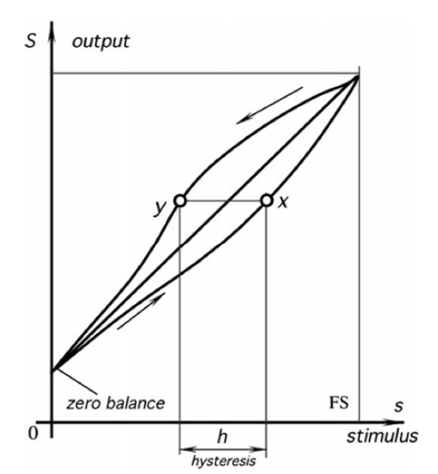
\includegraphics[scale=0.35]{img/hysteresis.png}
	\caption{Relation constitutive non univoque d'un matériau ferromagnétique :
	phénomène d'hystérèse.}
	\label{fig:hysteresis}
\end{figure}
La densité d'énergie magnétique étant donnée par
\begin{equation}
	W = \int \H \cdot \dif\B,
\end{equation}
on peut calculer la densité d'énergie totale durant un cycle complet
\[ W_\text{cycle} = \int_{B_r}^{-B_m} \H \cdot \dif\B 
+ \int_{-B_m}^{-B_r} \H \cdot \dif\B
+ \int_{-B_r}^{B_m} \H \cdot \dif\B
+ \int_{B_m}^{B_r} \H \cdot \dif\B \] 
et se rendre compte qu'elle est positive. %FIX: why?
La densité d'énergie perdue par cycle est proportionnelle à la surface du
cycle $W_\text{cycle} \propto S_\text{cycle}$ qui est elle
même $\propto B^2_m$.

La puissance totale perdue est donc donnée par
\begin{equation}
	P = fW_\text{cycle}V = K_hfVB^2_m
\end{equation}
où $f$ est la fréquence d'oscillation du champ magnétique,
$V$ le volume du matériau magnétique et $K_h$ une constante
propre au matériau.

\paragraph{Conductivité électrique non-nulle}
Chaque section du matériau magnétique intercepte lui aussi un flux
variable dans le temps. Par le loi de Faraday, une force électromotrice
apparait donc sur le contour de cette section
\[ e_{cm} = \fdif{}\Phi_{cm} \neq 0. \]
Si la conductivité du matériau magnétique est non-nulle, sa résistance
$R_{cm} \neq \infty$ et donc un courant $i_{cm} \neq 0$ apparaît. On les
appelle les courants de Foucault. Il est possible de réduire ces courants
en utilisant une superposition de tôles ferromagnétiques séparées par
un isolant à la place d'un seul bloc de matériau ferromagnétique. De la sorte,
on réduit la surface traversée par le flux variable.
Ces courants de Foucault engendre une perte de puissance
\begin{equation}
	P_\text{fouc} = R_{cm}I^2_{cm} = \frac{V^2_{cm}}{R_{cm}}.
\end{equation}
Comme en pratique on travaille avec des grandeurs sinusoïdales, on
peut dire que $\Phi_{cm} \propto B_m\cos(\omega t + \varphi)$ et
donc que $e_{cm} \propto \omega B_m$. On a donc finalement
\begin{equation}
	P_\text{fouc} = K_ff^2VB^2_m
\end{equation}
où $K_f$ est une constante propre au matériau et à l'épaisseur de tôle.

\paragraph{Pertes fer ou pertes magnétiques}
Les deux non-idéalités précédentes se regroupent dans ce qu'on
appelle les \emph{pertes fer} ou pertes magnétiques
\[ P_\text{fer} = P_\text{hyst} + P_\text{fouc}. \]

%FIX: je ne comprend pas comment on déduit ce modèlé àpd slide 25
\begin{figure}[ht!]
	\centering
	\includegraphics[scale=0.35]{img/mod-pertes-fer.png}
	\caption{Modélisation des pertes magnétiques.}
	\label{fig:mod-pertes-fer}
\end{figure}

\subsection{Circuit équivalent de référence}
Le circuit équivalent de référence du transformateur, aussi appelé
circuit en T du transformateur est donné en forme phasorielle à la figure
\ref{fig:mod-ref-transfo}. 

\begin{figure}[ht!]
	\centering
	\includegraphics[scale=0.35]{img/mod-ref-transfo.png}
	\caption{Circuit équivalent de référence ou circuit en T du
	transformateur.}
	\label{fig:mod-ref-transfo}
\end{figure}

Ce modèle ne tient pas compte 
\begin{itemize}
	\item des pertes par hystérésis et par courant de Foucault
	liées aux flux de fuite ;
	\item des effets péliculaires (effet de peau) dans les
	conducteurs des bobinages.
\end{itemize}
Néanmoins, on peut montrer que la modélisation de ces effets ne
changent pas la forme du schéma équivalent de référence. Les
paramètres du schéma équivalent ne peuvent donc pas être obtenus
directement par les formules présentées précédemment mais peuvent
par contre être identifiés par voie expérimentale.

%TODO : slide 28, modèle à inductances couplées

\subsection{Le transformateur en charge}
Pour un transformateur en charge, on sens les conventions utilisées
jusqu'ici pour adopter la convention présentée à à la figure
\ref{fig:conv-transfo-charge}. Les équations constitutives du
transformateurs changent donc quelques peu (un signe change).

\begin{figure}[ht!]
	\centering
	\includegraphics[scale=0.35]{img/conv-transfo-charge.png}
	\caption{Convention pour un transformateur en charge : une puissance
	positive correspond à une puissance entrante au primaire et sortante
	au secondaire.}
	\label{fig:conv-transfo-charge}
\end{figure}

\subsubsection{Identification des paramètres en charge}
On peut écrire la relation courant-tension du primaire et du secondaire
sous forme matricielle
\begin{equation*}
	\begin{pmatrix}
		\Up_1 \\ \Up2
	\end{pmatrix}
	=
	\begin{pmatrix}
		\Zp_{11} & \Zp_{12} \\
		\Zp_{21} & \Zp_{22}
	\end{pmatrix}
	\times
	\begin{pmatrix}
		\Ip_1 \\ -\Ip_2
	\end{pmatrix}.
\end{equation*}
FIXME : comment on obtient ces 6 équations?
Mais ce système ne fournit que 6 équations indépendantes étant donné
que $\Zp_{12} = \Zp_{21}$ et nous avons 7 paramètres à identifier
(les 6 éléments parasites et le rapport de transformation $k$). 
On va donc essayer de simplifier le schéma équivalent de référence
de la figure \ref{fig:mod-ref-transfo}.

\paragraph{Première simplification}
Une première simplfication consiste à permuter les élements séries
et les éléments parallèles du côté primaire. En faisant de la sorte,
on obtient le schéma de la figure \ref{fig:transfo-simpli-1}.

\begin{figure}[ht!]
	\centering
	\includegraphics[scale=0.35]{img/transfo-simpli-1.png}
	\caption{Première simplification du schéma équivalent de référence.}
	\label{fig:transfo-simpli-1}
\end{figure}

On obtient alors
\begin{align}
	\Zp_{po} 	& = \Zp_1 + \Zp_\mu &
	\Zp_1' 		& = \frac{\Zp_1 + \Zp_\mu}{\Zp_\mu} \Zp_1 &
	\bar{k}_s 	& = \frac{\Zp_1 + \Zp_\mu}{\Zp_\mu} k.
	\label{eq:transfo-charge-perm-serie-para}
\end{align}

On regroupe ensuite les éléments séries du côté secondaire pour
obtenir le circuit de la figure \ref{fig:transfo-simpli-1bis} où
\begin{align*}
	\Zp_e 		& = \frac{\Zp_1'}{\bar{k}^2_s} + \Zp_2 &
	\Up_{20} 	& = \frac{\Up_1}{\bar{k}_s}.
\end{align*}

\begin{figure}[ht!]
	\centering
	\includegraphics[scale=0.35]{img/transfo-simpli-1bis.png}
	\caption{Regroupement des éléments séries du côté secondaire.}
	\label{fig:transfo-simpli-1bis}
\end{figure}

\paragraph{Deuxième simplification}
On va maintenant supposer que le transformateur est proche du
transformateur idéal. Dans ce cas, on suppose que les effets des
éléments séries et parallèles sont petits et donc on peut les
étudier séparement. %FIXME : pourquoi?

On repart donc de du transformateur idéal avec notre nouvelle
convention (voir figure \ref{fig:transfo-charge-ideal}).

\begin{figure}[ht!]
	\centering
	\includegraphics[scale=0.35]{img/transfo-charge-ideal.png}
	\caption{Transformateur idéal avec la convention de charge.}
	\label{fig:transfo-charge-ideal}
\end{figure}

Avec cette convention, on a les relations suivantes
\begin{align*}
	\Ip_1 	& = \frac{\Ip_2}{k} &
	\Up_1 	& = k\Up_2
\end{align*}
ainsi que les bilans de puissances active et réactive
\begin{align*}
	\Re\{\Up_1\Ip_1^*\} & = \Re\{\Up_2\Ip_2^*\} &
	\Im\{\Up_1\Ip_1^*\} & = \Im\{\Up_2\Ip_2^*\}
\end{align*}
et la propriété de manipulation de circuit
\[ \frac{\Up_1}{\Ip_1} = k^2 \frac{\Up_2}{\Ip_2}. \]

\subparagraph{Effets des éléments parallèles}
On ajoute maintenant les éléments parallèles à la figure
\ref{fig:transfo-charge-ideal} pour étudier leurs effets.
Le circuit obtenu est présenté sur la figure \ref{fig:transfo-charge-para}.

\begin{figure}[ht!]
	\centering
	\includegraphics[scale=0.35]{img/transfo-charge-para.png}
	\caption{Effets des éléments parallèles par rapport au cas idéal.}
	\label{fig:transfo-charge-para}
\end{figure}

Par rapport au cas idéal, on a donc
\[ \Ip_1 = \frac{\Ip_2}{k} + \Ip_0. \]
On pourra alors négliger $\Ip_0$ si et seulement si
\[ \Ip_0 \ll \frac{\Ip_2}{k} \]
ce qui revient à dire que
\begin{equation}
	\Zp_\mu \gg k^2 \frac{\Up_2}{\Ip_2}
	\label{eq:transfo-charge-simpli-1}
\end{equation}
ou encore que
\begin{align*}
	X_\mu 	& \gg k^2 \frac{\Up_2}{\Ip_2} &
	R_{pm} 	& \gg k^2 \frac{\Up_2}{\Ip_2}.
\end{align*}

\subparagraph{Effets des éléments séries}
On ajoute maintenant les éléments séries à la figure
\ref{fig:transfo-charge-ideal}. Le circuit obtenu est
présenté à la figure \ref{fig:transfo-charge-series}.

\begin{figure}[ht!]
	\centering
	\includegraphics[scale=0.35]{img/transfo-charge-series.png}
	\caption{Effets des éléments séries par rapport au cas idéal. Tous
	les éléments séries ont été ramenés au secondaire.}
	\label{fig:transfo-charge-series}
\end{figure}

Par rapport au cas idéal, on a donc
\[ \Up_2 = \frac{\Up_1}{k} - (R_e + jX_e)\Ip_2. \]
On pourra alors négliger cette différece si et seulement si
\begin{equation}
	\Zp_e = R_e + jX_e \ll \frac{\Up_2}{\Ip_2}
	\label{eq:transfo-charge-simpli-2}
\end{equation} 
ou encore
\begin{align*}
	\frac{R_1}{k^2} 	& \ll \frac{U_2}{I_2} &
	\frac{X_1}{k^2}	& \ll \frac{U_2}{I_2} &
	R_2 				& \ll \frac{U_2}{I_2} &
	X_2				& \ll \frac{U_2}{I_2}	
\end{align*}

\subparagraph{Synthèse}
En combinant les équations \ref{eq:transfo-charge-simpli-1} et
\ref{eq:transfo-charge-simpli-2}, on arrive à la condition
\[ Z_e \ll \frac{U_2}{I_2} \ll \frac{Z_\mu}{k^2} \]
qui peut se réecrire de manière équivalente
\[ k^2Z_e \ll \frac{U_1}{I_1} \ll Z_\mu. \]
Si cette condition est respectée, alors les relations
\ref{eq:transfo-charge-perm-serie-para} deviennent
\begin{align*}
	\Zp_{po} 	& \approx \Zp_\mu &
	\Zp_1' 		& \approx \Zp_1 &
	\bar{k}_s 	& \approx k.
\end{align*}
Si le transformateur est proche d'un transformateur idéal, on peut donc 
en bonne approximation permuter les éléments parasites parallèles
et séries sans changer leurs valeurs ou la valeur de $k$.
On arrive finalement au schéma équivalent simplifié de la figure
\ref{fig:transfo-charge-eq-simpli} qui ne compte plus que 5 paramètres.
Les paramètres $X_e$ et $R_e$ sont donnés par
\begin{align*}
	X_e	& = \frac{\omega l_1}{k^2} + \omega l_2 &
	R_e	& = \frac{R_1}{k^2} + R_2.  
\end{align*}

\begin{figure}[ht!]
	\centering
	\includegraphics[scale=0.35]{img/transfo-charge-eq-simpli.png}
	\caption{Schéma équivalent simplifié du transformateur. En pratique,
	c'est celui qu'on utilise pour l'identification des paramètres.}
	\label{fig:transfo-charge-eq-simpli}
\end{figure}

\subsubsection{Caractéristique externe}
Si on ne s'intéresse qu'aux grandeurs de sortie $\Ip_2$ et $\Up_2$,
on peut utiliser le modèle équivalent de Thèvenin donné à la
figure \ref{fig:transfo-charge-mod-thevenin}. 

\begin{figure}[ht!]
	\centering
	\includegraphics[scale=0.35]{img/transfo-charge-mod-thevenin.png}
	\caption{Modèle équivalent de Thévenin, utilisé pour obtenir les
	caractéristiques de sortie du transformateur.}
	\label{fig:transfo-charge-mod-thevenin}
\end{figure}

%TODO : petit diagramme de Kapp correspondant (pour éviter le fond
quadrillé des slides...)
Via ce modèle, on obtient très facilement un diagramme de Kapp dans
lequel on peut appliquer pythagore généralisé
\[ U_{20}^2 = U_2^2 + 2U_2Z_eI_2\cos(\varphi_e - \varphi_2) + (Z_eI_2)^2. \]
En définissant le courant de court-circuit
\begin{equation}
	\Icc \eqdef \frac{U_{20}}{Z_e},
\end{equation}
on peut réecrire cette équation
\[ 1 = \left(\frac{U_2}{U_{20}}\right)^2 + 2\frac{U_2}{U_{20}}
\frac{I_2}{\Icc}\cos(\varphi_e - \varphi_2) + \left(\frac{I_2}{\Icc}\right)^2. \]
Cette dernière équation décrit différentes ellipses dans le plan
$(\frac{U_2}{U_{20}}, \frac{I_2}{\Icc})$ selon $\varphi_2$ (et donc selon
le type de charge).
TODO : refaire (ou trouver qqpart) les figures du slides 40 en meilleures qualités

Si les conditions \ref{eq:transfo-charge-simpli-1} et
\ref{eq:transfo-charge-simpli-2} sont respectées, alors on a aussi
\[ I_2 \ll \Icc. \]
Dans ce cas, on obtient finalement
FIXME : comment obtient-on ça?
\[ 1 = \frac{U_2}{U_{20}} + \frac{I_2}{\Icc}\cos(\varphi_e - \varphi_2) \]
ou encore
\[ U_2 = U_{20} - Z_eI_2\cos(\varphi_e - \varphi_2). \]

\subsection{Les essais}
Maintenant qu'on a obtenu un schéma équivalent simplifié (voir figure
\ref{fig:transfo-charge-eq-simpli}), analysons deux types
d'essais permettant d'identifier ses différents paramètres.

\subsubsection{En court-circuit}
Le principe (comme son nom l'indique) est d'alimenter un enroulement
alors que l'autre est en court-circuit. Qui dit court-circuit dit
courant élevé, et il faut donc travailler à des tensions bien inférieures
aux tensions nominales\footnote{La tension nominale est la tension de
fonctionnement normale du transformateur.} pour éviter de griller le
transformateur. En conséquence, les effets des éléments séries sont
prédominants.

\paragraph{Par le secondaire}
L'essai en court-circuit par le secondaire est illustré à la figure
\ref{fig:essai-cc-par-secondaire}. On peut déterminer l'amplitude
et la phase de l'impédance $\Zp_e$ via
\begin{align*}
	Z_e				& = \frac{U_2}{I_2} &
	\cos\varphi_e	& = \frac{P_2}{U_2I_2}.
\end{align*}
On retrouve ensuite les composantes $X_e$ et $R_e$ via l'équation
\ref{eq:imp-series-comp}.

\begin{figure}[ht!]
	\centering
	\includegraphics[scale=0.35]{img/essai-cc-par-secondaire.png}
	\caption{Essai en court-circuit par le secondaire.}
	\label{fig:essai-cc-par-secondaire}
\end{figure}

\paragraph{Par le primaire}
L'essai en court-circuit par le primaire est illustré à la figure
\ref{fig:essai-cc-par-primaire}. On peut déterminer l'amplitude
et la phase de l'impédance $\Zp'_e$ via
\begin{align*}
	Z'_e				& = \frac{U_1}{I_1} &
	\cos\varphi'_e	& = \frac{P_1}{U_1I_1}.
\end{align*}
où $\Zp'_e = k^2\Zp_e$. On retrouve ensuite les composantes $X_e$
et $R_e$ via l'équation \ref{eq:imp-series-comp}.

\begin{figure}[ht!]
	\centering
	\includegraphics[scale=0.35]{img/essai-cc-par-primaire.png}
	\caption{Essai en court-circuit par le primaire.}
	\label{fig:essai-cc-par-primaire}
\end{figure}

\subsubsection{\`{A} vide}
Dans ce type d'essai, un enroulement est alimenté alors que l'autre est
en circuit ouvert. On effectue en général ces tests à la tension
nominale et obtient des courants de loin inférieurs aux courants nominaux.
Dans ce cas, ce sont donc les éléments parallèles qui dominent.

\paragraph{Par le primaire}
L'essai à vide par le primaire est illustré à la figure
\ref{fig:essai-vide-primaire}. On détermine l'amplitude et la
phase de $\Zp_\mu$ en utilisant les relations
\begin{align*}
	Z_\mu 			& = \frac{U_1}{I_1} &
	\cos\varphi_\mu	& = \frac{P_1}{U_1I_1}
\end{align*}
avec $I_1 = I_0$ et $P_1 = P_0$. On retrouve ensuite les deux composantes
parallèles à l'aide de l'équation \ref{eq:imp-para-comp}. Comme de plus
$U_2 = U_{20}$, on a
\[ k = \frac{U_1}{U_{20}}. \]

\begin{figure}[ht!]
	\centering
	\includegraphics[scale=0.35]{img/essai-vide-primaire.png}
	\caption{Essai à vide par le primaire.}
	\label{fig:essai-vide-primaire}
\end{figure}

\begin{myrem}
	On choisit de faire l'essai à vide par le primaire ou par
	le secondaire selon le transformateur et les appareils de
	mesures disponibles. Par exemple, si on doit faire un essai
	à vide sur un transformateur abaisseur de tension dont la
	tension nominale d'entrée est de \SI{220}{\volt} et
	la tension nominale de sortie est de \SI{12}{\volt} et
	qu'on possède une petite source de tension ne pouvant pas
	dépasser les \SI{30}{\volt}, on fera bien évidemment l'essai
	à vide par le secondaire. 
\end{myrem}

\begin{myrem}
Lorsqu'on effectue un essai, on mesure aussi la puissance active.
Dans le cas d'essai en court-circuit, celle-ci correspond
aux pertes par effet Joules. Tandis que dans le cas d'essai en
circuit-ouvert, celle-ci correspond aux pertes fer.
\end{myrem}

\subsubsection{Retour au circuit de référence}

À partir des éléments du circuit simplifié ($R_{pm}$, $X_\mu$,
$R_e$ et $X_e$), on peut revenir au circuit de référence, qui
a une interprétation physique plus directe. Pour cela, il faut
faire des hypothèses supplémentaires, par exemple:
\[ X_1 = X_2' \Rightarrow
	\left\{
		\begin{aligned}
			X_1 &= \frac{X_e'}{2} \\
			X_2' &= \frac{X_e'}{2}
		\end{aligned}
	\right.
\]

Pour les résistances série: on mesure séparément les résistances
en DC: $R_{1,DC}$, $R_{2, DC}$. On fait ensuite l'approximation
\[ \frac{R_1}{R_2} = \frac{R_{1,DC}}{R_{2,DC}} \Rightarrow
	\left\{
		\begin{aligned}
			R_1 &\approx
			\frac{R_e'}{R_{1,DC}+k^2 R_{2,DC}} R_{1, DC} \\
			R_2 &\approx
			\frac{R_e'}{R_{1,DC}+k^2 R_{2,DC}} R_{2, DC}
		\end{aligned}
	\right.
\]

\subsubsection{Améliorations}

On peut utiliser les valeurs des éléments série (calculés via
l'essai en court-circuit) pour améliorer la précision des
éléments parallèles. Lors de l'essai à vide:
\begin{gather*}
	\bar{Z_\mu} = \bar{Z_0} - R_1 - jX_1 \\
	k = \frac{Z_\mu}{Z_0}\frac{U_1}{U_{20}}
\end{gather*}

Ces approximations sont valables uniquement si $Z_1 \ll Z_0$.

\begin{myrem}
	On ne fait pas l'inverse (utiliser l'essai à vide pour
	améliorer la précision de l'essai en court-circuit car ce
	dernier s'effectue à une tension largement inférieure à la
	tension nominale, et donc le niveau de saturation est plus
	faible qu'à tension nominale, la valeur de $R_{pm}$ est
	donc très différente.
\end{myrem}

\subsection{Caractéristiques}

\subsubsection{Valeurs nominales}

Ces valeurs sont inscrites sur la plaquette signalétique du tansformateur
(voir exemple fig.~\ref{fig:plaquette-signaletique-transfo}).

Elles sont toujours exprimées en valeur efficace et correspondent à un
fonctionnement normal du dispositif.

\begin{figure}
	\centering
	\includegraphics[width=0.3\textwidth]{img/plaquette-signaletique-transfo.png}
	\caption{Plaquette signalétique d'un transformateur (triphasé).}
	\label{fig:plaquette-signaletique-transfo}
\end{figure}

\paragraph{Tension nominale}
Par exemple, $U_{1N} = \SI{230}{V}$.

Si on dépasse cette valeur, comme $U_1 \propto \omega B_m$ et
$P_{fer} \propto B_m^2$, le transformateur va surchauffer.
Il y a aussi un effet de saturation du matériau magnétique ($\mu$
diminue), ce qui augmente $I_1$ (on modélise ça par une diminution
de $X_\mu$). Par conséquent les pertes joule augmentent, ce qui
accentue la surchauffe.

\begin{myrem}
	Une surchauffe \og modérée\fg du transformateur affecte sa durée
	de vie, principalement via un veillissement plus rapide des
	isolants (en plastique...) des câbles. Si la surchauffe est
	importante, elle peut causer un incendie (durée de vide \emph{très}
	réduite.
\end{myrem}

\paragraph{Fréquence nominale}
Typiquement \SI{50}{Hz} ou \SI{60}{Hz}.

Si $f>f_N$, $R_{pm}$ diminue et donc les pertes fer et joule augmentent.

% TODO justifier pourquoi R_{pm} diminue quand f augmente

\paragraph{Tension secondaire norminale}
Elle n'est pas choisie, elle dépend directement de la tension primaire
nominale et du rapport de transformation.

Suivant les normes, elle correspond à la tension à vide: $U_2 = U_{2N}$
lorsque $U_1 = U_{1N}$ et $I_2 = 0$.

\paragraph{Courant secondaire nominale}
Comme $P_{Joule} \propto I^2$, on a ici aussi un risque de surchauffe
en cas de dépassement de la valeur nominale.

Cette valeur est rarement indiqueé.

\paragraph{Puissance secondaire nominale}
Il s'agit de la puissance apparente, donc on déduit le courant
secondaire nominal:
\[I_{2N} = \frac{S_{2N}}{U_{2N}}\]

On donne la puissance apparente car il est impossible de connaitre
le facteur de puissance de la charge à l'avance, et la grandeur
utile est en fait le courant nominal (c'est lui qui est limité
physiquement, pas la puissance activée qui passe par le transfo).

\paragraph{Courant et puissance primaires nominales}

Souvent on ne les spécifie pas, on suppose le transformateur idéal:
\[S_{1N} = S_{2N} = S_N.\]
Le courant secondaire nominal vaut donc
\[I_{1N} = \frac{S_N}{I_{2N}}.\]
À condition que $I_0 \ll I_{1N}$ et $Z_e I_{2N} \ll U_{2N}$.

\subsubsection{Valeurs de court-circuit}

\paragraph{Courant de court-circuit}
C'est le courant qui circule dans un enroulement lorsque cet
enroulement est court-circuité et que la tension nominale est
appliquée à l'autre enroulement.

Généralement ce courant est très grand ($I_{cc} \gg I_N$), on ne
peut donc pas le mesurer directement, on le calcule via les équations
\begin{align*}
	I_{2cc} &= \frac{U_{2N}}{Z_e} \\
	I_{1cc} &= \frac{U_{1N}}{Z_e'}
\end{align*}

\paragraph{Tension de court-circuit}
Tension qu'il faut appliquer à un enroulement pour qu'y circule un
courant égal au courant nominal, lorsque l'autre enroulement est
court-circuité.

Généralement $U_{cc} \ll U_N$, on peut donc le mesurer sans problèmes;
cela correspond à un essai en court-circuit avec $I = I_N$.

On peut utiliser le courant de court-circuit pour déterminer l'impédance
série du schéma équivalent: \[Z_e = \frac{U_{2cc}}{I_{2N}}.\]

\subsubsection{Pertes}

\paragraph{Pertes \og magnétiques\fg}
\[P_{fer} \approx \frac{U_1^2}{R_p}\]
Appelées aussi pertes fixes, car elles sont indépendantes de la charge.

\paragraph{Pertes \og par effet Joule\fg}
\[P_{Joule} = R_1 I_1^2 + R_2 I_2^2 \approx R_e I_2^2\]
avec \[R_e = \frac{R_1}{k^2} + R_2.\]

Ces pertes sont donc proportionnelles aux carré du courant, absorbé
par la charge, on les appelle aussi pertes dues à la charge.

\subsubsection{Rendement}

Par définition,
\[\eta = \frac{P_2}{P_1}
	= \frac{P_2}{P_2 + P_{pertes}}
	= \frac{U_2 I_2 \cos\phi}{U_2 I_2 \cos\phi + P_{fer} + P_{Joule}}\]

Pour une tension primaire fixée, on peut calculer le rendement optimum
(en supposant que la tension au secondaire reste constante):
\[\fpart{\eta}{I_2} = 0 \Rightarrow P_{fer} = P_{Joule}.\]

En pratique, lors de la conception, on cherche à fixer le courant
nominal pour vérifer cette condition.

\subsection{Divers}

\subsubsection{Possibilité de déphasage}

Si on inverse les bornes en sortie du transformateur, on ajoute un
déphasage de \SI{180}{\degree}.

\subsubsection{Mise en parallèle de deux transformateurs}

\begin{figure}[ht!]
	\centering
	\includegraphics[width=0.5\textwidth]{img/parallele-transfos-mono.png}
	\caption{Mise en parallele de deux transformateurs.}
%	\label{fig:transfo-parallele}
\end{figure}

Mettre deux transformateurs en parallèle permet d'additioner leurs
puissances apparentes: $S_{tot} \approx S_A + S_B$, mais il faut
respecter certaines conditions:

\begin{itemize}
	\item Les tensions secondaires à vide doivent être identiques,
		donc les rapports de transformation doivent être égaux:
		\[k_A = k_B\]
	\item Les enroulements doivent être connectés dans le même sens
		par rapport aux bornes de référence.
	\item Les déphasages introduits par les transformateurs doivent
		être identiques: \[\phi_{2A} = \phi_{2B}\]
\end{itemize}

Si ces conditions ne sont pas satisfaites, il y aura un courant à vide
dans les transformateurs (rapidement très élevé... et donc desctructeur).

De plus, si on veut pouvoir utiliser efficacement les deux transformateurs,
il faux que la puissance passant par les transformateurs soit
proportionnelle à leur puissance nominale, ce qui revient à imposer
\[U_{2ccA} = U_{2ccB}.\]

On peut rattraper un petit déséquilibre avec un transformateur
d'équilibrage, présenté à la figure~\ref{fig:eq-transfo-parallele}.

\begin{figure}[ht!]
	\centering
	\includegraphics[width=0.5\textwidth]{img/eq-transfo-parallele}
	\caption{Équilibrage de transformateurs mis en parallèle.}
	\label{fig:eq-transfo-parallele}
\end{figure}

\subsubsection{Transformateur à prises multiples}

\begin{figure}[ht!]
	\centering
	\includegraphics[width=0.5\textwidth]{img/transfo-prises-multiples}
	\caption{Transformateur à prises multiples.}
	\label{fig:transfo-prises-multiples}
\end{figure}

Les transformateurs à prises multiples (fig.~\ref{fig:transfo-prises-multiples})
permet d'adapter la tension de sortie en modifiant le nombre effectif de
spires au secondaire.

Cela est utile notamment lorsque une charge variable est séparée du
transformateur par une ligne résistive: en faisant varier la tension
à la sortie du transformateur, on garde la tension constante à la charge
(ex.: distribution d'électricité dans un quartier).

Diverses techiques permettent de changer la tension sans couper
l'alimentation de la charge.

\subsubsection{Autotransformateurs}

\begin{figure}[ht!]
	\centering
	\includegraphics[width=0.5\textwidth]{img/autotransfo-mono.png}
	\caption{Autotransformateur à rapport de transformation variable.}
	\label{fig:autotransfo-mono}
\end{figure}

Les autotransformateurs (voir fig.~\ref{fig:autotransfo-mono})
utilisent le même enroulement pour le primaire et le
secondaire. Cela permet de faire des économies de fil électrique (d'autant plus
que les courants primaires et secondaires sont de signes opposés, l'amplitude
de la somme est donc réduite).

\subsection{Sécurité}

Toucher un seul conducteur suffit souvent pour être traversé par un courant,
même s'il s’agit du neutre.
En effet, il existe souvent un chemin possible entre l'autre conducteur et
la terre même si l'une des arrivées est coupée.

Un transformateur normal assure une isolation galvanique entre le réseau et
l'utilisateur. On peut dans ce cas toucher un conducteur sans risquer d'être
traversé par un courant. Il suffit d'ajouter un simple interrupteur au
primaire pour qu'il n'y ait plus de tension au secondaire.

Les autotransformateurs n'apportent pas ces garanties, car il n'y a pas
d'isolation galvanique. Le secondaire reste dangereux, même si la tension
est amenée à zéro avec le transformateur, ou si le primaire est coupé avec
un simple interrupteur.

\subsection{Aspects constructifs}

Le volume des deux enroulements est en général semblable. En effet, pour
avoir la même puissance dissipée: $I_1^2 R_1 = I_2^2 R_2$, et donc
\[\frac{n_1 \rho}{S_1} = \frac{n_2 \rho}{S_2} \left(\frac{I_2}{I_1}\right)^2.\]
Sachant que $I_2/I_1 = n_1/n_2$, on trouve
\[n_1 S_1 = n_2 S_2\]

Il peut toutefois y avoir plus d'isolant du côté haute tension.


\section{Le transformateur triphasé}

\subsection{Systèmes triphasés}

\begin{myrem}
	Cette partie est très proche du cours de circuits et mesures
	(ELEC1370), le contenu ici est très résumé.
\end{myrem}

\subsubsection{Phases}

Il y a trois phases, avec un courant et une tension associés. Il y a
deux types de systèmes:
\begin{itemize}
\item Système direct
	\begin{align*}
u_a &= \sqrt{2}U_{ph,a}\cos\left(\omega t+\phi_u\right) &
i_a &= \sqrt{2}I_{ph,a}\cos\left(\omega t+\phi_i\right) \\
u_b &= \sqrt{2}U_{ph,b}\cos\left(\omega t+\phi_u - \frac{2\pi}{3}\right) &
i_b &= \sqrt{2}I_{ph,b}\cos\left(\omega t+\phi_i - \frac{2\pi}{3}\right) \\
u_c &= \sqrt{2}U_{ph,c}\cos\left(\omega t+\phi_u - \frac{4\pi}{3}\right) &
i_c &= \sqrt{2}I_{ph,c}\cos\left(\omega t+\phi_i - \frac{4\pi}{3}\right)
	\end{align*}
\item Système inverse
	\begin{align*}
u_a &= \sqrt{2}U_{ph,a}\cos\left(\omega t+\phi_u\right) &
i_a &= \sqrt{2}I_{ph,a}\cos\left(\omega t+\phi_i\right) \\
u_b &= \sqrt{2}U_{ph,b}\cos\left(\omega t+\phi_u + \frac{2\pi}{3}\right) &
i_b &= \sqrt{2}I_{ph,b}\cos\left(\omega t+\phi_i + \frac{2\pi}{3}\right) \\
u_c &= \sqrt{2}U_{ph,c}\cos\left(\omega t+\phi_u + \frac{4\pi}{3}\right) &
i_c &= \sqrt{2}I_{ph,c}\cos\left(\omega t+\phi_i + \frac{4\pi}{3}\right)
	\end{align*}
\end{itemize}

On passe d'un système inverse à un système direct (et vice-versa) en
échangeant deux phases. Plus mathématiquement, on peut aussi prendre
l'opposé de la fréquence.

\begin{myrem} La suite des développements se fera avec un système
	direct (convention par défaut en électrotechnique).
\end{myrem}

Si $U_{ph,a} = U_{ph,b} = U_{ph,c}$, on parle de système équilibré pour
les tensions (idem pour les courants).

\subsubsection{Puissance}

\begin{align*}
	p_a &= u_a i_a
	= P_a + S_a \cos\left(2\omega t + \phi_u + \phi_i\right) \\
	p_b &= u_b i_b
	= P_b + S_b \cos\left(2\omega t + \phi_u + \phi_i - \frac{4\pi}{3}\right) \\
	p_c &= u_c i_c
	= P_c + S_c \cos\left(2\omega t + \phi_u + \phi_i - \frac{2\pi}{3}\right) 
\end{align*}

On a toujours $P_i \leq S_i$ (égalité ssi $\phi_u = \phi_i$).

Si le système est équilibré en tension et en courant, $P_a = P_b = P_c$
et $S_a = S_b = S_c$. On a alors
\[p = p_a + p_b + p_c = 3P = 3U_{ph}I_{ph}\cos\phi\]
où $\phi = \phi_u - \phi_i$.
On voit ici un intérêt des systèmes triphasés équilibrés: \textbf{la puissance
est constante}.

\subsubsection{Phaseurs}
On suit la convention générale en électrotechnique.
Si le système est équilibré, et soit $\bar{a} = e^{j2\pi/3}$,

%TODO : switch to summarry conventions :
% \bar{U} --> \Up
\begin{align*}
	\bar{U} &= U_{ph}e^{j\phi_u}
	& \bar{U_a} &= \bar{U}
	& \bar{U_b} &= \bar{a}^2\bar{U}
	& \bar{U_c} &= \bar{a}\bar{U} \\
	\bar{I} &= I_{ph}e^{j\phi_i}
	& \bar{I_a} &= \bar{I}
	& \bar{I_b} &= \bar{a}^2\bar{I}
	& \bar{I_c} &= \bar{a}\bar{I} \\
\end{align*}

\begin{align*}
	\bar{S_{3\phi}}
	&= \bar{U_a}\bar{I_a}^* +
	\bar{U_b}\bar{I_b}^* +
	\bar{U_c}\bar{I_c}^* \\
	&= \bar{U}\bar{I}^* +
	\bar{a}^2\bar{U}\bar{a}^{-2}\bar{I}^* +
	\bar{a}\bar{U}\bar{a}^{-1}\bar{I}^* \\
	&= 3\bar{U}\bar{I}^* \\
	P_{3\phi} &= \Re{(\bar{S_{3\phi}})} = 3UI\cos\phi \\
	Q_{3\phi} &= \Im{(\bar{S_{3\phi}})} = 3UI\sin\phi \\
\end{align*}

\subsubsection{Liaisons}

\begin{itemize}
	\item Connection \og naïve\fg: 6 fils.
	\item En mutualisant le neutre: 4 fils.
	\item Si le système est équilibré le courant dans le neutre
		est nul: 3 fils restants.
\end{itemize}

Un système triphasé équilibré transfert donc trois fois plus de puissance
qu'un système monophasé, avec deux fois moins de fils et deux fois
moins de pertes (vu qu'il y a deux fois moins de fils, et le courant
dans les fils restants est le même que pour les systèmes monophasés).

\subsubsection{Grandeurs de ligne et de phase}

\begin{myrem}
	En électrotechnique, on parle par défaut de grandeurs de ligne.
\end{myrem}

La notion de grandeur de ligne et de grandeur de phase dépend du
point de vue: liaison ou charge.

\paragraph{Côté liaison}
\begin{itemize}
	\item Courant de ligne et courant de phase (identique):
		courant sur un des fils de la liaison.
	\item Tension de ligne: tension entre deux phases
		(entre deux fils).
	\item Tension de phase: tension entre une phase et le
		neutre (même s'il n'y a pas de fil de neutre).
\end{itemize}

\begin{figure}[ht!]
	\centering
	\includegraphics[width=0.5\textwidth]{img/grandeurs-ligne-phase-liaison.png}
	\caption{Grandeurs de phase et de ligne, vu côté liaison.}
	\label{fig:grandeurs-ligne-phase-liaison}
\end{figure}

En utilisant les conventions de la figure~\ref{fig:grandeurs-ligne-phase-liaison},
on trouve successivement
\begin{align*}
	\bar{U_{RN}} &= \bar{U_{ph}} \\
	\bar{U_{SN}} &= \bar{U_{ph}}e^{-j2\pi/3} \\
	\bar{U_{RS}} &= \bar{U_{ligne}} = \bar{U_{ph}}\left(1-e^{-j2\pi/3}\right) \\
	\bar{U_{ligne}} &= \sqrt{3}\bar{U_{ph}}e^{j\pi/6}.
\end{align*}

On a alors les puissances triphasées:
\[P = p = 3U_{ph}I_{ph}\cos\phi\]
donc, comme $U_{ligne} = \sqrt{3}U_{ph}$ et $I_{ligne} = I_{ph}$,
\[P = p = \sqrt{3}U_{ligne}I_{ligne}\cos\phi\]

On a la même relation pour $Q$ et $S$ (en adaptant le facteur de
puissance, $\sin\phi$ ou $1$).

\paragraph{Côté dispositif}
Le dispositif est constitué de trois impédances montées en triangle ou
en étoile. Ces impédances sont appelées phases du dispositif. La relation
entre les grandeurs de phase côté dispositif et les grandeurs de phase et
de ligne côté liaison dépendent du type de connexion du dispositif.

\subparagraph{Connexion étoile}
\begin{align*}
	\bar{U}_{ph,dispositif} &= \bar{U}_{ph,liaison}
		= \frac{1}{\sqrt{3}}\bar{U}_{ligne}e^{-j\pi/6} \\
	\bar{I}_{ph,dispositif} &= \bar{I}_{ph,liaison} = \bar{I}_{ligne}
\end{align*}


\subparagraph{Connexion triangle}
\begin{align*}
	\bar{U}_{ph,dispositif} &= \bar{U}_{ligne} = \sqrt{3}\bar{U}_{ph,liaison}e^{j\pi/6} \\
	\bar{I}_{ph,dispositif} &= \frac{1}{\sqrt{3}}\bar{I}_{ph,liaison}e^{j\pi/6}
		= \frac{1}{\sqrt{3}}\bar{U}_{ph,liaison}e^{j\pi/6} \\
\end{align*}

\subsubsection{Circuit équivalent monophasé}

On peut ne considérer qu'une seule des trois phases, avec
typiquement
\begin{align*}
	\bar{U} &= \bar{U_a} \\
	\bar{I} &= \bar{I_a}.
\end{align*}

On peut l'interpréter comme le circuit qui, juxtaposé à deux autres
circuits identiques \emph{non couplés}, permet de reproduire le
comportement du dispositif triphasé.

\begin{myrem}
	Par convention, le circuit équivalent est définit par rapport
	aux grandeurs de phase côté liaison.

	Cela permet de calculer des schémas équivalents en ne
	connaissant que des mesures sur la ligne, et rien de la charge.
\end{myrem}

On a donc pour la puissance
\begin{align*}
	S_{3\phi} &= 3UI\\
	P_{3\phi} &= 3UI\cos\phi\\
	Q_{3\phi} &= 3UI\sin\phi
\end{align*}

\begin{myrem}[Charges couplées] Dans le cas où les éléments associés
	aux phases de la charge sont couplés entre eux, on ne peut pas
	prendre la valeur sur une seule phase pour trouver le circuit
	équivalent (cela reviendrait à négliger le couplage).
	Par exemple, dans le cas d'inductances couplées
	(voir fig.~\ref{fig:charge-tri-couplee}), on calcule
	\begin{align*}
		U_a &= L_p \fdif{i_a}{t} + M \fdif{i_b}{t} + M \fdif{i_c}{t} \\
		    &= (L_p-M)\fdif{i_a}{t} \qquad\text{car $i_a+i_b+i_c=0$}
	\end{align*}
	On a donc $L_{eq} = L_p-M$.
	\begin{figure}[ht!]
		\centering
		\includegraphics[width=0.5\textwidth]{img/charge-tri-couplee.png}
		\caption{Charge triphasée avec couplage entre les phases.}
		\label{fig:charge-tri-couplee}
	\end{figure}
\end{myrem}

\paragraph{Représentation d'une charge}
Comme le circuit équivalent est défini par rapport aux grandeurs de phase côté
liaison, le schéma équivalent change si on change le type de connection de la
charge.

Dans le cas où la charge est constituée des trois impédances montées en
étoile, si ces impédances ne sont pas couplées alors l'impédance du
circuit équivalent est celle d'une des phases.

Les circuits équivalents sont les suivants (en utilisant les
relations entre grandeurs de phase côté liaison et côté charge):
\begin{center}
\includegraphics[width=0.4\textwidth]{img/charge-tri-etoile.png}
\includegraphics[width=0.4\textwidth]{img/eq-tri-etoile.png}
\end{center}
\begin{center}
\includegraphics[width=0.4\textwidth]{img/charge-tri-triangle.png}
\includegraphics[width=0.4\textwidth]{img/eq-tri-triangle.png}
\end{center}

On peut aussi simplifier le circuit en utilisant les relations pour 
passer d'une impédance triangle en impédance étoile. Cette relation
est (dans le cas d'une charge équilibrée):
\[
  \bar{Z}_{triangle} = 3\bar{Z}_{étoile}
\]

\subsubsection{Valeurs nominales}

Par convention, les grandeurs nominales sont les grandeurs vues de la
liaison:
\begin{itemize}
	\item Tension nominale: tension de ligne
	\item Courant nominal: courant de ligne
	\item Puissance nominale: puissance triphasée
\end{itemize}

Si un système permet deux types de connexion physique, il y a deux
jeux de grandeurs nominales (sauf pour la puissance, qui est constante).

\subsubsection{Dispositions pratiques}

Certains borniers permettent de choisir le type de connexion:
\begin{itemize}
	\item Connexion en étoile:
		\begin{center}
			\includegraphics[width=0.4\textwidth]{img/bornier-etoile.png}
		\end{center}
	\item Connexion en triangle:
		\begin{center}
			\includegraphics[width=0.4\textwidth]{img/bornier-triangle.png}
		\end{center}
\end{itemize}

%TODO transformateur triphasé : slides 31 à 41 


\part{Les convertisseurs électromécaniques}

% Cette section est-t'elle vraiment utile?
\section{Introduction générale}
\begin{mydef}[Conversion électromécanique]
Une conversion électromécanique d'énergie est une transformation
d'une énergie mécanique en énergie électrique et réciproquement.
\end{mydef}

\begin{mydef}[Convertisseur électromécanique]
Un convertisseur électromécanique est un dispositif au sein
duquel on exploite les \textbf{couplages} qui peuvent se produire
entre des phénomènes \textbf{électriques} et des phénomènes
\textbf{mécaniques}.
\end{mydef}

\subsection{Classification}
\subsubsection{Selon le principe de fontionnement}
\paragraph{Couplage via le champ magnétique}
Lorsque le champ magnétique est responsable du couplage, on parle
de convertisseurs électromagnétiques.

\begin{itemize}
	\item Un conducteur de longueur $l$ parcouru par un courant $i$
	et plongé dans un champ magnétiqu $B$ subit une force égale à $Bli$.
	Réciproquement, un conducteur de longueur $l$ se déplaçant dans
	un champ $B$ à une vitesse $v$ voit apparaître à ses extrémités
	une différence de potentiel égale à $Blv$. On parle alors de
	\textbf{force électrodynamique}.
	\item Un corps ferromagnétique plongé dans un champ $B$ subit
	une force qui l’attire vers une position maximisant le flux
	magnétique produit. Réciproquement, la variation de flux associé au
	déplacement du corps ferromagnétique induit une force
	électromotrice au sein de la spire qui génère le champ.
	On parle alors de \textbf{force réluctante}.
\end{itemize}

%TODO pour "à large cycle" (cfr. slide 11)
Pour générer le champ magnétique, on utilise des aimants permanents ou
des électroaimants.

\paragraph{Couplage via le champ électrique}
Lorsque le champ électrique est responsable du couplage, on parle
de convertisseurs électrostatiques.\\

\begin{itemize}
	\item Un corps portant une charge $q$ et plongé dans un champ
	électrique $E$ subit une force $qE$. Réciproquement, un corps chargé
	se déplaçant dans un champ électrique $E$ voit son potentiel
	électrique varier.
	\item Un corps diélectrique plongé dans un champ électrique $E$
	subit une force qui l’attire vers une position maximisant le
	flux électrique produit. Réciproquement, la variation de flux associé
	au déplacement du corps diélectrique induit une variation de
	charge (un courant) au niveau des électrodes qui génèrent
	le champ électrique $E$.
\end{itemize}

\paragraph{Couplage piézoélectrique - magnétostrictif}
On utilise ici les propriétés intrinsèques de certains matériaux.
Un matériaux piésoélectrique est un matériau qui voit apparaître une
différence de potentiel à ses bornes lorsqu'on le comprime.

\subsubsection{Selon la fonction}
\paragraph{Convertisseurs d'énergie}
Lorsqu'on convertit de l'énergie mécanique en énergie électrique, on
parle de \textbf{générateurs}. A l'inverse, lorsqu'on convertir de
l'énergie électrique énergie mécanique, on parle de \textbf{moteurs}.

Il s'agit de convertisseurs de type électromagnétiques avec les
caractéristiques suivantes :
\begin{itemize}
	\item Rendement de conversion élevé ;
	\item Fonctionnement à puissance constante ;
	\item Interconnectables.
\end{itemize}

\paragraph{Actionneurs}
Un actionneurs est un convertisseurs conçu pour assurer la commande
de systèmes mécaniques à partir de grandeurs électriques imposées.
Ils peuvent être de chaque type (électromagnétique, électrostatiques,
piézoélectriques-magnétostrictif) et présentent les caractéristiques
suivantes :
\begin{itemize}
	\item Facilité et précision de la commande en couple ou en force ;
	\item Couple ou force massique élevés ;
	\item Rendement élevé ;
	\item Connecté à une source d'énergie électrique au travers d'un
	convertisseur électronique de puissance.
\end{itemize}

\paragraph{Capteurs}
Un capteur a pour but de transformer de mesurer des grandeurs mécaniques
en les transformant en signaux électriques.
Le type de convertisseur dépend cette fois du type de grandeur à mesurer
et de la gamme de mesure.

\section{Théorie générale}
\subsection{Structure}
Un convertisseur électromécanique est constitué :
\begin{itemize}
	\item d'un élément fixe : le stator ;
	\item d'un élément mobile : le rotor ;
	\item et d'un dispositif de guidage qui détermine le mouvement
	du rotor par rapport au stator.
\end{itemize}

\begin{myexem}
	Sur le haut-parleur de la figure \ref{fig:example-conv-struct}, le
	noyau et l'aimant permanent constitue le stator, l'enroullement mobile
	constitue le rotor et c'est la membrane élastique qui assure le guidage.

	\begin{figure}[ht!]
		\centering
		\includegraphics[width=0.5\textwidth]{img/example-conv-struct.png}
		\caption{Structure d'un haut-parleur.}
		\label{fig:example-conv-struct}
	\end{figure}
\end{myexem}

De manière générale, la structure d'un convertisseur
électromécanique est représentée sur la figure \ref{fig:conv-struct-general}.

\begin{figure}[ht!]
	\centering
	\includegraphics[width=0.65\textwidth]{img/conv-struct-general.png}
	\caption{Structure générale d'un convertisseur électromécanique.}
	\label{fig:conv-struct-general}
\end{figure}

\subsection{Hypothèses de base}
\paragraph{Electriques}
\begin{myhyp}
Les conducteurs sont toujours assimilables à des bobinages
pour chacun desquels on peut définir :
\begin{itemize}
	\item Un courant qui y circule ;
	\item Une tension à ses bornes.
\end{itemize}
\label{hyp:conv-elec-cond}
\end{myhyp}

\begin{myhyp}
Les phénomènes d'hystérésis et les courants induits dans
les matériaux magnétiques sont négligés.
\end{myhyp}

\paragraph{Mécaniques}
\begin{myhyp}
Les corps sont supposés rigides.
\end{myhyp}

\begin{myhyp}
Le rotor ne possède qu'un seul degré de liberté.
\end{myhyp}

\subsection{Equations électriques}
Pour chaque conducteur $k \in [1, n]$ de résistance $R_k$ et assimilable
à une bobine (hypothèse \ref{hyp:conv-elec-cond}), la loi de
Faraday s'écrit
\begin{equation}
	u_k = R_ki_k + \fdif{\Psi_k}{t}
	\label{eq:general-faraday}
\end{equation}
où
\begin{equation}
	\Psi_k 					= \Psi_k(i_1, i_2, \dots, i_k, \dots, i_n, \theta_m)
	\Leftrightarrow i_k		= i_k(\Psi_1, \Psi_2, \dots, \Psi_k, \dots, \Psi_n,
	\theta_m).  
\end{equation}
On a donc une relation univoque dépendant de la géométrie, des
matériaux et de la position ($\theta_m$ ici).

\paragraph{Cas linéaire}
L'inductance mutuelle entre le conducteur $i$ et le conducteur $j$ est donnée
dans le cas linéaire par
\begin{equation}
	L_{ij} = \frac{\Psi_i}{i_j}\bigg|_{i_k=0}, \forall k \neq j.
\end{equation}
On peut donc réecrire
\begin{equation}
	\Psi_k(i_1, i_2, \dots, i_k, \dots, i_n, \theta_m) = \sum_{j=1}^n
	L_{kj}(\theta_m)i_j
	\label{eq:linear-i-phi-relation}
\end{equation}
et enfin
\begin{equation}
	u_k = R_ki_k + \sum_{j=1}^n L_{kj}\fdif{i_j}{t} + 
	\fdif{\theta_m}{t}\sum_{j=1}^n\fpart{L_{kj}}{\theta_m}i_j.
\end{equation}

\paragraph{Cas non-linéaire}
Dans le cas non-linéaire, l'inductance mutuelle est donnée par
\begin{equation}
	L_{v,ij} = \fpart{\Psi_i}{i_j}\bigg|_{i_k=0}, \forall k \neq j
\end{equation}
où l'indice $v$ est pour \og variationnel \fg{}. Dans ce cas, on a
\begin{equation}
	L_{v,ij} = R_ki_k + \sum_{j=1}^n L_{v,kj}\fdif{i_j}{t} + 
	\fdif{\theta_m}{t}\fpart{\Psi_k}{\theta_m}.
\end{equation} 

\subsection{Energie et co-énergie magnétique}
\subsubsection{Energie magnétique}
L'énergie magnétique peut s'exprimer de manière équivalente
de plusieurs façons
\begin{equation}
	% FIX : comment passer de int H dB à int F dPhi ?
	W_{\text{mag}} = \int H\dif B = \int \MMF\dif\Phi = \int i\dif\Psi. 
\end{equation}
en utilisant les relations suivantes
\begin{align*}
	\Phi & = \int_S \B\cdot\dS & \MMF & = \int_\Gamma \H\cdot\dl 
\end{align*}
pour passer de l'énergie associée aux champs magnétiques à l'énergie
associée au flux magnétique et
\begin{align*}
	\Psi & = n\Phi & \MMF & = ni
\end{align*}
pour passer de l'énergie associée aux flux magnétiques à l'énergie
associée aux flux magnétiques encerclés par les enroullements.
L'énergie magnétique est représentée sur la figure \ref{fig:energie-magn-phi-i}
en fonction de $\Psi$ et $i$.

\begin{figure}[ht!]
	\centering
	\includegraphics[width=0.35\textwidth]{img/energie-magn-phi-i.png}
	\caption{Energie magnétique dans un repère $(i, \Psi)$ (le graphe est 
	identique pour les autres repères).}
	\label{fig:energie-magn-phi-i}
\end{figure}

\subsubsection{Bilan énergétique d'un convertisseur}
Calculons le bilan énergétique d'un convertisseur électromécanique sur un
intervalle de temps $\dif t$ et pour une position $\theta_m$ donnée. Un tel
convertisseur est représentée d'un point de vue énergétique à la figure
\ref{fig:bilan-energie-general}. Sous ces hypothèses, les énergies électriques
(qui sont les seules non-nulles avec l'énergie magnétique stockée dans
le convertisseur) sont données par
\begin{align*}
	\dif W_{\text{élec}} & = \sum_{k=1}^n u_ki_k\dif t
	\stackrel{\text{éq. \ref{eq:general-faraday}}}{=} \sum_{k=1}^n R_ki^2_k\dif t
	+ \sum_{k=1}^n i_k\dif\Psi_k \\
	\dif W_{\text{pertes élec}} &= \sum_{k=1}^n R_ki^2_k\dif t \text{ (pertes joules)}
\end{align*}

\begin{figure}[ht!]
	\centering
	\includegraphics[width=0.4\textwidth]{img/bilan-energie-general.png}
	\caption{Bilan d'énergie d'un convertisseur sous les hypothèses du
	convertisseur électromagnétique et pour une position fixée. Les énergies
	grisées sont nulles sous ces hypothèses.}
	\label{fig:bilan-energie-general}
\end{figure}
On trouve ensuite l'énergie magnétique stockée dans le convertisseur en
appliquant la conservation de l'énergie
\begin{equation}
	\dif W_{\text{élec}} = \dif W_{\text{pertes élec}} + \dif W_{\text{mag}}
\end{equation}
ce qui permet d'obtenir
\begin{equation}
	\dif W_{\text{mag}} = \sum_{k=1}^n i_k\dif\Psi_k.
\end{equation}
L'énergie magnétique totale est donc donnée par
\begin{align*}
	W_{\text{mag}} 	& = \int_{0,0,\dots,0}^{\Psi_1,\Psi_2,\dots,\Psi_n}
	\sum_{k=1}^n i_k(\Psi_1,\Psi_2,\dots,\Psi_n,\theta_m)\dif\Psi_k \\
					&= W_{\text{mag}}({\Psi_1,\Psi_2,\dots,\Psi_n,\theta_m})
\end{align*}
% FIX : j'aurais dis dW/dPhi_i = dW/dPhi_j ?
L'énergie étant une fonction d'état, on a
\begin{equation}
	\fpart{\Psi_j}{i_k} = \fpart{\Psi_k}{i_j}
\end{equation}
ce qui dans le cas linéaire comme dans le cas non-linéaire implique
\begin{equation}
	L_{(v),kj} = L_{(v),jk}.
\end{equation}

\subsubsection{Co-énergie magnétique}
\begin{mydef}[Co-énergie magnétique]
La co-énergie magnétique est définie comme
\begin{equation}
	W_{\text{cmag}} = \sum_{k=1}^n i_k\Psi_k - W_{\text{mag}}.
\end{equation}
Graphiquement, cette définition est illustrée sur la figure
\ref{fig:co-energie-magn}.
\end{mydef}
\begin{figure}[ht!]
	\centering
	\includegraphics[width=0.4\textwidth]{img/co-energie-magn.png}
	\caption{Illustration graphique de la co-énergie magnétique.}
	\label{fig:co-energie-magn}
\end{figure}
A partir de la définition, on obtient
\begin{equation}
	\dif W_{\text{cmag}} = \sum_{k=1}^n (i_k\dif\Psi_k + \dif i_k\Psi_k)
	- \dif W_{\text{mag}}.
\end{equation}
En utilisant ensuite les résultats du bilan d'énergie, on obtient
\begin{equation}
	\dif W_{\text{cmag}} = \sum_{k=1}^n \Psi_k\dif i_k.
\end{equation}
A nouveau, la co-énergie magnétique totale est donc donnée par
\begin{align*}
	W_{\text{cmag}} 	& = \int_{0,0,\dots,0}^{i_1,i_2,\dots,i_n}
	\sum_{k=1}^n \Psi_k(i_1,i_2,\dots,i_n,\theta_m)\dif i_k \\
					&= W_{\text{cmag}}({i_1,i_2,\dots,i_n,\theta_m})
\end{align*}
et est aussi une fonction d'état. Dans le cas linéaire pour lequel
on a l'équation \ref{eq:linear-i-phi-relation}, on peut réecrire
cette denière relation comme
\begin{equation}
	W_{\text{cmag}} = \frac{1}{2}\sum_{k=1}^n\sum_{j=1}^n L_{kj}i_ki_j.
\end{equation}
L'avantage de cette réecriture et qu'elle permet de réecrire la
co-énergie magnétique comme un produit matriciel
\begin{equation}
	W_{\text{cmag}} = \frac{1}{2}\mathbf{I}^T\mathbf{L}(\theta_m)\mathbf{I}
	\label{eq:co-energie-matriciel}
\end{equation}
où
\begin{equation}
	\mathbf{I} = [i_1, i_2, \dots, i_n]^T
\end{equation}
est la matrice des courants et $\mathbf{L}$ est la matrice des inductances.



%CONTINUATION 9/4/2018



\subsection{Couple électromagnétique}

Reprenons l'expression du bilan d'énergie sur un intervalle de temps $dt$ mais cette fois-ci pour une  position $\theta$ variable :


\begin{align*}
	\dif W_{\text{élec}} &= \dif W_{\text{pertes élec}} + \dif W_{\text{mag}} + \dif W_{\text{em}} \\	
	\xcancel{\sum_{k=1}^n R_k\ i_k^2 \dif t} + \sum_{k=1}^n i_k\ \dif \Psi_k &= \xcancel{\sum_{k=1}^n R_k\ i_k^2 \dif t} \\
	&+ \sum_{k=1}^n \frac{\partial W_{\text{mag}}}{\partial \Psi_k} + \frac{\partial W_{\text{mag}}}{\partial \theta_m} \dif \theta_m \\
	&+ C_{em} \dif \theta_m
\end{align*}

\begin{figure}[ht!]
	\centering
	\includegraphics[width=0.5\textwidth]{img/bilansurdtslide29.png}
	\caption{Bilan d'énergie d'un convertisseur sous les hypothèses du
	convertisseur électromagnétique. Les énergies
	grisées sont nulles sous ces hypothèses.}
	\label{fig:bilan-energie-general-theta-variable}
\end{figure}

On a donc pour des $\Psi_k$ et $\theta_m$ indépendants:
\begin{equation}
\underbrace{\sum_{k=1}^n i_k\ \dif \Psi_k = \sum_{k=1}^n \frac{\partial W_{\text{mag}}}{\partial \Psi_k} \dif \Psi_k } + \underbrace{\frac{\partial W_{\text{mag}}}{\partial \theta_m} \dif \theta_m + C_{em} \dif \theta_m}
\end{equation}

\begin{align}
i_k &= \frac{\partial W_{\text{mag}}}{\partial \Psi_k}	
&
C_{em} &= \frac{\partial W_{\text{mag}}}{\partial \theta_m}
\end{align}

On peut faire le même raisonnement avec $\dif W_{\text{mag}} = \sum_{k=1}^n (i_k \dif \Psi_k + \Psi_k \dif i_k) - \dif W_{\text{cmag}}$

\begin{align*}	
	\xcancel{\sum_{k=1}^n R_k\ i_k^2 \dif t} + \xcancel{\sum_{k=1}^n i_k\ \dif \Psi_k} &= \xcancel{\sum_{k=1}^n R_k\ i_k^2 \dif t} \\
	&+ \sum_{k=1}^n ( \xcancel{i_k \dif \Psi_k} + \Psi_k \dif i_k) -  \sum_{k=1}^n \frac{\partial W_{\text{cmag}}}{\partial i_k} \dif i_k - \frac{\partial W_{\text{cmag}}}{\partial \theta_m} \dif \theta_m \\
	&+ C_{em} \dif \theta_m
\end{align*}

On a donc pour des $i_k$ et $\theta_m$ indépendants:
\begin{equation}
\underbrace{0 = \sum_{k=1}^n \Psi_k \dif i_k -  \sum_{k=1}^n \frac{\partial W_{\text{cmag}}}{\partial i_k} \dif i_k} \underbrace{-\frac{\partial W_{\text{cmag}}}{\partial \theta_m} \dif \theta_m + C_{em} \dif \theta_m}
\end{equation}
\begin{align}
\Psi_k &= \frac{\partial W_{\text{cmag}}}{\partial i_k} 
&
C_{em} &= \frac{\partial W_{\text{cmag}}}{\partial \theta_m} 
\end{align}

En utilisant l'équation \ref{eq:co-energie-matriciel} on peut réécrire le couple $C_{em} =\frac{1}{2}\mathbf{I}^T \frac{\partial \mathbf{L}(\theta_m)}{\partial \theta_m}\mathbf{I} $

Lorsque les convertisseurs présentent des aimants permanents, les expressions précédentes sont modifiées:

\begin{align*}
W_{\text{mag}}({\Psi_1,\Psi_2,\dots,\Psi_n,\theta_m}) 	& = W_{\text{mag0}}(\theta_m) + \int_{0,0,\dots,0}^{\Psi_1,\Psi_2,\dots,\Psi_n}
	\sum_{k=1}^n i_k(\Psi_1,\Psi_2,\dots,\Psi_n,\theta_m)\dif\Psi_k \\
	W_{\text{cmag}}({i_1,i_2,\dots,i_n,\theta_m}) 	& = W_{\text{cmag0}}(\theta_m) + \int_{0,0,\dots,0}^{i_1,i_2,\dots,i_n}
	\sum_{k=1}^n \Psi_k(i_1,i_2,\dots,i_n,\theta_m)\dif i_k 					
\end{align*}
\vspace{-4ex}
\begin{figure}[ht!]
	\centering
	\includegraphics[width=0.25\textwidth]{img/co-energie-magn-aimant.png}
	\label{fig:co-energie-magn-aimant}
\end{figure}

\vspace{-4ex}
\begin{align*}
&\downarrow ( \Psi_k(i_1,i_2,\dots,i_k,\dots,i_n,\theta_m) = \Psi_{k0}(\theta_m) = + \sum_{j=1}^n L_{jk}(\theta_m)i_j ) \\
W_{\text{cmag}}({i_1,i_2,\dots,i_n,\theta_m}) &= W_{\text{cmag0}}(\theta_m) + \sum_{k=1}^n \Psi_{k0}(\theta_m) i_k + \frac{1}{2} \sum_{k=1}^n\sum_{j=1}^n L_{kj}(\theta_m) i_k i_j \\
&\downarrow C_{em} = \frac{\partial W_{\text{cmag}}}{\partial \theta_m} \\
\Aboxed{C_{em} &= \underbrace{\frac{\partial W_{\text{cmag0}}(\theta_m)}{\partial \theta_m}}_{\text{couple de détente}} + \underbrace{\sum_{k=1}^n \frac{\partial \Psi_{k0}(\theta_m)}{\partial \theta_m} i_k}_{\text{couple électrodynamique}} + \underbrace{\frac{1}{2} \sum_{k=1}^n\sum_{j=1}^n \frac{\partial L_{kj}(\theta_m)}{\partial \theta_m}  i_k i_j}_{\text{couple réluctant}}}
\end{align*}


\begin{figure}[ht!]
	\centering
	\includegraphics[width=0.7\textwidth]{img/couples.png}
	\caption{Classification des couples électromagnétiques}
\end{figure}

\section{Les machines à champ tournant}

\subsection{Structure}

\subsubsection{Enroulements}

Les machines à champ tournant sont composées d'enroulements à p paires de pôles. Les conducteurs aller-retour sont alors espacés de $180/p\ ^\circ $.Un enroulement génère p pôles nord et p pôles sud et enfin, les enroulements statoriques et rotoriques doivent posséder le même nombre de paires de
pôles.

\subsubsection{Relation flux - courants}

Un certain nombre d'hypothèses sur la structure d'une machine à champ tournant sont nécessaires afin de simplifier les calculs:
\begin{itemize}
\item Les enroulements sont remplacés par un conducteur situé à l'interface rotor-entrefer ou
stator-entrefer.
\item La perméabilité magnétique des circuits statoriques et rotoriques est supposée infinie.
Le champ magnétique est donc nul en dehors de l'entrefer.
\item L'entrefer est mince par rapport au rayon. Cela implique un champ magnétique radial
dans l'entrefer qui ne dépend pas du rayon.
\item Les effets de bords sont supposés négligeables. (étude 2D)
\item Pour le calcul des inductances propres et mutuelles, on considère les aimants permanents
comme de l'air.
\end{itemize}
\vspace{0.5cm}

Par la loi d'ampère $\oint \vec H . \vec dl = N i$, on a pour un contour $ABCD$ n'entourant aucun courant, \\


\begin{multicols}{2}
\noindent
\[ \oint_{ABCD} \vec H. \vec dl = H_e(\theta_1) e' - H_e(\theta_2) e' = 0 \] \[\frac{B_e(\theta_1)}{\mu_0}e' - \frac{B_e(\theta_2)}{\mu_0}e' = 0 \] \[B_e(\theta_1) = B_e(\theta_2) \]
En prenant un contour $ABCD$ entourant un courant entrant, \[ \oint_{ABCD} \vec H. \vec dl = H_e(\theta_1) e' - H'_e(\theta_2) e' = Ni \] \[\frac{B_e(\theta_1)}{\mu_0}e' - \frac{B_e'(\theta_2)}{\mu_0}e' = Ni \] 
On suppose par symétrie que $B_e(\theta_1) = -B_e'(\theta_2)$\[H_e(\theta_1) = \frac{B_e(\theta_1)}{\mu_0} = \frac{Ni}{2e'} \] 
\vfill\null
\columnbreak
\noindent
\begin{Figure}
    \centering
	\includegraphics[width=0.7\textwidth]{img/flux-courant.png}
\end{Figure}

\end{multicols}

Lorsqu'on développe l'expression du champ en séries de Fourier, on constate que le champ $\vec{H_e}$ est constitué d'une composante sinusoïdale  ainsi que d'harmoniques, que l'on voudrait minimiser pour obtenir un champ le plus sinusoïdal possible. Cela est rendu possible grâce à l'étalement sur un angle $\alpha$ qui dépend de $p$ et avec un nombre $m$ d'encoches:

\begin{multicols}{2}
\noindent
\begin{Figure}
    \centering
	\includegraphics[width=0.7\textwidth]{img/etalement1.png}
\end{Figure}
\vfill\null
\columnbreak
\begin{Figure}
    \centering
	\includegraphics[width=0.9\textwidth]{img/etalement2.png}
	\captionof{figure}{Tableau des amplitudes relatives des différentes harmoniques pour $\alpha=60^\circ$}
\end{Figure}
\end{multicols}

\newpage

%\samepage{
\subsubsection*{inductance propre}
\begin{multicols}{2}
\noindent
Le flux vaut $\phi = \int_S \vec B . d \vec S$ on a donc 
\begin{align*}
\phi &= R_e L_z \int_{\theta_0 - \pi/2}^{\theta_0 + \pi/2} B_e(\theta) d\theta \\
&= R_e L_z \int_{\theta_0 - \pi/2}^{\theta_0 + \pi/2}{ \mu_0 \frac{Ni}{2e' } d\theta} \\
&= \mu_0 \frac{Ni \pi R_e L_z}{2e'}
\end{align*}
Puisque $\psi = N\phi$ et $L = \psi / i$ on a \[L = \mu_0 \frac{N^2 \pi R_e L_z}{2e'} \]

\vfill\null
\columnbreak
\noindent
\begin{Figure}
    \centering
	\includegraphics[width=\textwidth]{img/indu-propre.png}
\end{Figure}
\end{multicols}
%}

\subsubsection*{inductance mutuelle}
Les inductances mutuelles peuvent être calculées : \[  \begin{array}{l} M_{21} = M_0 \left( 1 - 2 \frac{\theta_{21}}{\pi} \right) 

\end{array} \ \ \  \ M_0 = \mu_0 \frac{N_1 N_2 \pi R_e L_z}{2e'} \]

En récapitulant on peut donner les relations suivantes :
\begin{multicols}{2}
\noindent
Situation idéale:
\begin{align*}
L_1 &= \mu_0 \frac{N_1^2 \pi R_e L_z}{2e'}\\
L_2 &= \mu_0 \frac{N_2^2 \pi R_e L_z}{2e'}\\
M_0 &= \mu_0 \frac{N_1 N_2 \pi R_e L_z}{2e'} \\
L_1 &= \frac{N_1}{N_2}M_0 & L_2 &= \frac{N_2}{N_1}M_0\\
\frac{L_1}{L_2} &= \frac{N_1^2}{N_2^2} & M_0^2&=L_1\ L_2
\end{align*}
\vfill\null
\columnbreak
\noindent
Situation réelle:
\vspace{-2ex}
\begin{align*}
L_1 &= \mu_0 \frac{N_1^2 \pi R_e L_z}{2e'}+l_1 = L_{10}+l_1\\
L_2 &= \mu_0 \frac{N_2^2 \pi R_e L_z}{2e'}+l_2 = L_{20}+l_2\\
M_0 &= \mu_0 \frac{N_1 N_2 \pi R_e L_z}{2e'}+m_0 \\
\end{align*}
avec : $0<l_1<<L_{10}$

\end{multicols}
On peut donc définir un \textbf{coefficient de dispersion :} \[\sigma = 1 - \frac{M_0^2}{L_1L_2} \]

\subsubsection{Cas des systèmes triphasés}
\begin{multicols}{2}
\noindent
\begin{Figure}
    \centering
	\includegraphics[width=0.5\textwidth]{img/triphase.png}
	\captionof{figure}{}
\end{Figure}
\vfill\null
\columnbreak
\noindent
Caractéristiques:
\begin{itemize}
\item
Décallés de $120 ^\circ$ électriques:
$$\left\{
\begin{array}{l}
  \theta_{ea} = \theta_{e0} \\
  \theta_{eb} = \theta_{e0} + 2\pi/3 \\
  \theta_{ec} = \theta_{e0} + 4\pi/3 
\end{array}
\right.$$

\item
\textbf{ Harmonique d'ordre trois du champ
total d'entrefer disparaît} si :
$$i_a+i_b+i_c=0$$
\end{itemize}
\end{multicols}

%TODO autres structures

\subsection{Principe de fonctionnement}

\subsubsection{Structure de base}

\begin{multicols}{2}
\noindent
\begin{Figure}
    \centering
	\includegraphics[width=0.5\textwidth]{img/triphase-struc.png}
	\captionof{figure}{}
\end{Figure}
\vfill\null
\columnbreak
\noindent
\begin{itemize}
\item Convertisseur rotatif
\item Stator et rotor concentriques
\item Pôles lisses
\item Systèmes triphasés d’enroulements
\item Paires de pôles p
\item Etalement sur 2.m encoches t.q. chaque enroulement occupe $120^\circ$ électriques
\end{itemize}
\end{multicols}

\subsubsection{Equations}

\begin{figure}[ht!]
	\centering
	\includegraphics[width=0.6\textwidth]{img/triphase-equa.png}
\end{figure}
Hypothèse champs sinusoïdaux, cas idéal:
$$
\left\{
\begin{array}{l}
  M_{sa-ra} = M_{sb-rb} = M_{sc-rc} = M_{sr}.\cos(\theta_m) \\
  M_{sa-rb} = M_{sb-rc} = M_{sc-ra} = M_{sr}.\cos(\theta_m + 2\pi/3) \\
  M_{sa-rc} = M_{sb-ra} = M_{sc-rb} = \underbrace{M_{sr}.\cos(\theta_m +4\pi/3)}_{\text{couplage sin parfait}} \\
\end{array}
\right.
M_{sr} = \underbrace{\frac{4\mu_0 N_s N_r R_e L_z}{p^2 \pi e'}}_{\text{répartition sinus}} \ \underbrace{\frac{\sin(\pi/6)}{m_s\ \sin(\pi/6\ m_s)}}_{\text{étalement stator}}\ \underbrace{\frac{\sin(\pi/6)}{m_r\ \sin(\pi/6\ m_r)}}_{\text{étalement rotor}} $$
$$
\left\{
\begin{array}{l}
L_s = \frac{N_s}{N_r}\ \frac{m_r\sin(\pi/6\ m_r)}{m_s\sin(\pi/6\ m_s)}\ M_{sr} \\
M_s = L_s.\ \cos(2\pi/3) = -1/2 L_s
\end{array}
\right.
\left\{
\begin{array}{l}
L_r = \frac{N_r}{N_s}\ \frac{m_s\sin(\pi/6\ m_s)}{m_r\sin(\pi/6\ m_r)}\ M_{sr} \\
M_r = L_r.\ \cos(2\pi/3) = -1/2 L_r
\end{array}
\right.
$$
\begin{multicols}{2}
\noindent
Cas général:
\begin{align*}
u_{sk} &= R_{sk}.i_{sk}+\frac{\Psi_{sk}}{dt}\\
u_{rk} &= R_{rk}.i_{rk}+\frac{\Psi_{rk}}{dt}\\
\end{align*}
\vfill\null
\columnbreak
\noindent
Cas linéaire:
\vspace{-1ex}
\begin{align*}
\Psi_{sa} &= L_s.i_{sa} + M_s.i_{sb} + M_s.i_{sc} &+ M_{sr}.\cos(\theta_{em}).i_{ra} \\
& &+ M_{sr}.\cos(\theta_{em}+2\pi/3).i_{rb}\\
& &+ M_{sr}.\cos(\theta_{em}+4\pi/3).i_{rc}\\
\end{align*}
\end{multicols}

\newpage
\subsubsection{Alimentation}
\begin{multicols}{2}
\noindent
\textbf{stator}:\\
Système direct:
$$\left\{
\begin{array}{l}
  i_{sa} = \sqrt{2}.i_s.cso(\omega_st+\phi_s)\\
  i_{sb} = \sqrt{2}.i_s.cso(\omega_st+\phi_s - 2\pi/3)\\
  i_{sc} = \sqrt{2}.i_s.cso(\omega_st+\phi_s - 4\pi/3)\\
\end{array}
\right.$$
\vfill\null
\columnbreak
\noindent
\textbf{rotor}:\\
Système direct:
$$\left\{
\begin{array}{l}
  i_{sa} = \sqrt{2}.i_s.cso(\omega_st+\phi_s)\\
  i_{sb} = \sqrt{2}.i_s.cso(\omega_st+\phi_s - 2\pi/3)\\
  i_{sc} = \sqrt{2}.i_s.cso(\omega_st+\phi_s - 4\pi/3)\\
\end{array}
\right.$$
Système inverse:
$$\left\{
\begin{array}{l}
  i_{sa} = \sqrt{2}.i_s.cso(\omega_st+\phi_s)\\
  i_{sb} = \sqrt{2}.i_s.cso(\omega_st+\phi_s + 2\pi/3)\\
  i_{sc} = \sqrt{2}.i_s.cso(\omega_st+\phi_s + 4\pi/3)\\
\end{array}
\right.$$
\end{multicols}

\noindent

En développant les équations citées ci-dessus dans l'expression du couple électromagnétique, on peut obtenir l'expression suivante :
\begin{align}
C_{em} &= \frac{9}{2}.p.M_{sr}.I_s.I_r.\sin(\omega_st-\omega_rt-\theta_{em}+\phi_s - \phi_r)\\
&\downarrow \theta_{em} = p.\omega_m.t + \theta_{e0} \\
&= \frac{9}{2}.p.M_{sr}.I_s.I_r. \underbrace{\sin( (\omega_s-\omega_r-p.\omega_m).t}_{\text{valeur moyenne nulle}} + \phi_s - \phi_r - \theta_{e0} )
\end{align}

\begin{myrem}
Le couple électromagnétique est bien du type \textbf{électrodynamique} !
\end{myrem}

Afin de supprimer le terme fluctuant à valeur moyenne nulle, les relations suivantes sont requises :
Pour une alimentation sinusoïdale, on a \[ \begin{array}{l} \text{Système direct} \\ \text{Système inverse}
\end{array} \ \ \ \begin{array}{l}
\omega_s - \omega_r - p \omega_m = 0 \\ \omega_s + \omega_r - p \omega_m = 0
\end{array} \  \ \ \Rightarrow \ \ \ \begin{array}{l}
\omega_r = \omega_s - p \omega_m \\ \omega_r = -\omega_s + p \omega_m 
\end{array} \]

Le couple électromagnétique est alors, \[ C_{em} = \frac{9}{2} p.M_{sr}. I_s. I_r. \sin (\varphi_s - \varphi_r - \theta_{e0} ) \]

Et la co-énergie magnétique est \textbf{constante} ! \[ W_{cmag} = \frac{3}{2} L_{cs} I_s^2 + \frac{3}{2} L_{cr} I_r^2 + \frac{9}{2} M_{sr} I_s I_r \cos (\varphi_s - \varphi_r - \theta_{e0} ) \]
où $L_{cs}$ et $L_{cr}$ sont les inductances cycliques ($L_s - M_s$ et $L_r - M_r$)

\subsubsection{Schéma équivalent}

En développant les équations suivantes, on peut obtenir un schéma équivalent pour les machines à champ tournant triphasées.
\begingroup
\large
\begin{equation}
\left\{
\begin{array}{l}
  \mathbf{U}_s = \mathbf{R}_s.\mathbf{I}_s + \frac{d}{dt}[ \mathbf{L}_s.\mathbf{I}_s + \mathbf{M}_{sr}(\theta_{em}).\textbf{I}_r] \\
    \mathbf{U}_r = \mathbf{R}_r.\mathbf{I}_r + \frac{d}{dt}[ \mathbf{L}_r.\mathbf{I}_r + \mathbf{M}_{sr}^T(\theta_{em}).\textbf{I}_s] \\
\end{array}
\right.
\left\{
\begin{array}{l}
\bar{V}_s = R_s \bar{I}_s + j\ \omega_s.l_{cs}.\bar{I}_s + j\ \omega_s.k.\frac{3}{2}.M_{sr}.\left( \bar{I}_s + \frac{1}{k}.e^{j\ \theta_{e0}}.\bar{I}_r \right) \\
\bar{V}_r = R_r \bar{I}_r + j.( \omega_s - p.\omega_m).l_{cr}.\bar{I}_r \\
\hspace{1cm} + j( \omega_s - p.\omega_m).\frac{1}{k}.\frac{3}{2}.M_{sr}.\left( \bar{I}_r + k.e^{-j\ \theta_{e0}}.\bar{I}_s \right) \\
\end{array}
\right.
\label{eq: u=ri+...}
\end{equation}
 \endgroup
 
\begin{figure}[H]
	\centering
	\includegraphics[width=0.8\textwidth]{img/schema-equi.png}
	\caption{Schéma équivalent d'une machine à champ tournant en triphasé}
\end{figure}
Les courants magnétisants représentent un système triphasé de courants statoriques qui produiraient à eux seuls le champ magnétique d'entrefer généré par les
courants statoriques et rotoriques. Ou encore des courants qui produiraient les mêmes FEM aux bornes des enroulements statoriques et rotoriques.
$$ \bar{I}_\mu  = \bar{I}_s + \frac{1}{k}. e^{j.\theta_{e0}}.\bar{I}_r$$

%TODO Calcul du couple électromagnétique via la loi $B.L.I$
%TODO Calcul des tensions induites via la loi $B.L.V$
\subsubsection{Prise en compte de la saturation}

Nous pouvons à présent prendre en compte la saturation des matériaux ferromagnétiques. Celle-ci influence uniquement les inductances dont le circuit magnétique est
formé de ces matériaux. On ne prendra donc pas les inductances de fuite en compte. Le niveau de saturation dépend du niveau de champ dans le matériau et donc indirectement, du courant
magnétisant, ou encore de la FEM.\\
L'inductance est donc remplacée par une inductance dépendante du courant qui la traverse:
\begin{align*}
M_{sr} &= f(I_\mu) &ou & & M_{sr} &= f(E)
\end{align*}


\subsubsection{Marche en machine synchrone et asynchrone}

On parle de machine asynchrone lorsque la rotation du rotor n'est pas en phase avec la pulsation des courants du stator (voir prochaine section). La machine synchrone au contraire génère un champ magnétique constant au rotor à l'aide de courants constants ou d'aimants permanents. Ceci a pour effet de faire tourner le rotor à la même vitesse que les pulsations du stator.

\[ \boxed{\omega_s - \omega_r - p.\omega_m =0 } \]

\begin{multicols}{2}
\noindent
%\textbf{Synchrone}
\begin{align*}
\omega_r &= 0 & \omega_m &= \omega_s/p
\end{align*}
\begin{Figure}
    \centering
	\includegraphics[width=0.9\textwidth]{img/synchrone.png}
	\captionof{figure}{Marche en machine synchrone}
\end{Figure}
\vfill\null
\columnbreak
\noindent
%\textbf{Asynchrone}
\begin{align*}
p.\omega_m \neq \omega_s &&&& \omega_r &= \omega_s - p.\omega_m
\end{align*}
\begin{Figure}
    \centering
	\includegraphics[width=0.9\textwidth]{img/asynchrone.png}
	\captionof{figure}{Marche en machine asynchrone}
\end{Figure}
\end{multicols}


\section{La machine asynchrone}

\subsection{Conditions d'utilisation}

\subsubsection*{connexion au réseau :}
Le système triphasé sortant du réseau est défini comme : \[ \left\{ \begin{array}{l}
e_a = \sqrt{2} V_{\infty} \cos (\omega_ \infty t + \psi _{\infty} )  \\
e_b = \sqrt{2} V_{\infty} \cos (\omega_ \infty t + \psi _{\infty} - 2\pi /3) \\
e_c = \sqrt{2} V_{\infty} \cos (\omega_ \infty t + \psi _{\infty} - 4\pi /3)
\end{array} \right. \]

\subsubsection*{Équation mécanique}

\[C_{em} - C_p - C_r = J_t \frac{d\omega_m}{dt} \]
où $C_{em}$ est le couple électromagnétique, $C_p$ est le couple des pertes, $C_r$ est le couple du rotor (couple utile) et $J_t$ est le moment d'inertie.

\begin{myhyp}
On fait l'hypothèse que la constante de temps électrique << constante de temps mécanique
\end{myhyp}

\subsection{Dispositions constructives particulières}

Il existe deux types de machines asynchrones:
\begin{multicols}{2}
\noindent
\begin{Figure}
    \centering
	\includegraphics[width=0.6\textwidth]{img/rotor-bobine.png}
	\captionof{figure}{Machine à rotor bobiné}
\end{Figure}
\vfill\null
\columnbreak
\noindent
\begin{Figure}
    \centering
	\includegraphics[width=0.6\textwidth]{img/cage-ecu.png}
	\captionof{figure}{machine à rotor à cage d'écureuil}
\end{Figure}
\end{multicols}
\noindent

Les machines à rotor à cage sont appelées comme tel car les enroulements rotoriques sont en fait court-circuités aux extrémités de la cage par une plaque conductrice.


\subsection{Équations}

En développant les équations matricielles \ref{eq: u=ri+...}, on arrive aux résultats suivants:\\
\noindent
\textbf{Stator}:
\begin{equation*}
\begin{array}{l}
\bar{V}_s = R_s \bar{I}_s + j\ \omega_s.l_{cs}.\bar{I}_s + j\ \omega_s.k.\frac{3}{2}.M_{sr}.\left( \bar{I}_s + \frac{1}{k}.e^{j\ \theta_{e0}}.\bar{I}_r \right)
\end{array}
\left\{
\begin{array}{l}
\bar{V}_s = V_s.e^{j.\Psi_s} \\
\bar{I}_s = I_s.e^{j.\phi_s} \\
\end{array}
\right.
\left\{
\begin{array}{l}
L_{cs} = L_s - M_s = k.\frac{3}{2}.M_{sr}+l_{cs} \\
L_s = \frac{N_s}{N_r}\ \frac{m_r.\sin(\pi/6\ m_r)}{m_s.\sin(\pi/6\ m_s)}
\end{array}
\right.
\end{equation*}
\textbf{Rotor} :
\begin{equation*}
0 = R_r \bar{I}_r + j.( \omega_s - p.\omega_m).l_{cr}.\bar{I}_r + j( \omega_s - p.\omega_m).\frac{1}{k}.\frac{3}{2}.M_{sr}.\left( \bar{I}_r + k.e^{-j\ \theta_{e0}}.\bar{I}_s \right)
\left\{
\begin{array}{l}
\bar{V}_s = V_s.e^{j.\Psi_s} \\
\bar{I}_s = I_s.e^{j.\phi_s} \\
\end{array}
\right.
L_{cr} = L_r - M_r = k.\frac{3}{2}.M_{sr}+l_{cr} 
\end{equation*}
\noindent
\textbf{Couple électromagnétique}
$$C_{em} = \Im{\left\{ \frac{9}{2}.p.M_{sr}.\bar{I}_s. \left( \bar{I}_s.e^{j.\theta_{e0}} \right)^* \right\} }$$
\noindent
\textbf{Connexion au réseau}
\begin{align*}
\omega_s &= \omega_{\infty} \\
\bar{V}_s &= \bar{V}_{\infty} - j.\omega_{\infty}.l_g.\bar{I}_s &\rightarrow \bar{V}_s \simeq \bar{V}_{\infty}
\end{align*}

En introduisant les notations,

\begin{align*}
L_\mu &= k.\frac{3}{2}.M_{sr} & \bar{I}_r' &= -\frac{1}{k}. e^{j.\theta_{e0}}.\bar{I}_r \\
R_r' &= k^2.R_r \\
l_{cr}' &= k^2.l_{cr} & \gamma &= \frac{\omega_{\infty}/p - \omega_m}{\omega_{\infty}/p} = \frac{\omega_{\infty} - p.\omega_m}{\omega_{\infty}}
\end{align*}

On aboutit aux équations finales:
\begin{align}
C_{em} &= - \Im{ \left\{ 3.p.L_\mu.\bar{I}_s.\bar{I}_r'^* \right\} } \numberthis \label{eq: C-im}
\\
\bar{V}_{\infty} &\stackrel{\textbf{ST}}{=} R_s.\bar{I}_s + j.\omega_{\infty} .l_{cs}.\bar{I}_s + j.\omega_{\infty}.L_\mu .(\bar{I}_s - \bar{I}_r' ) \\
j.\omega_{\infty}.L_\mu.(\bar{I}_s - \bar{I}_r') = &\stackrel{\textbf{RO}}{=} \frac{R_r'}{\gamma}. \bar{I}_r' + j.\omega_{\infty}.l_{cr}'.\bar{I}_r'
\end{align}
\subsection{Schéma équivalent}

Ces équations constitutives peuvent être implémentées en un schéma équivalent qu'on ramène au stator afin de simplifier au maximum le circuit. On a donc :

\begin{figure}[H]
	\centering
	\includegraphics[scale=0.5]{img/schema-equi-asynch-non-simpl.png}
	\caption{Schéma équivalent d'une machine asynchrone ramené au stator (non-simplifié)}
\end{figure}

que l'on peut ensuite simplifier par :

\begin{figure}[H]
	\centering
	\includegraphics[scale=0.5]{img/schema-equi-asynch-simpl.png}
	\caption{Schéma équivalent d'une machine asynchrone ramené au stator}
	\label{fig:schema-equi-asynchrone}
\end{figure}

\subsection{Diagramme vectoriel}

Le diagramme de Kapp dérivant de ce schéma simplifié de la machine asynchrone est présenté ici :

\begin{figure}[H]
	\centering
	\includegraphics[scale=0.25]{img/diag-en-cercle.png}
	\caption{Diagramme vectoriel du schéma équivalent - "en cercle"}
\end{figure}

\subsection{Caractéristique couple-vitesse}

\subsection*{Puissance mécanique}

La puissance mécanique est donnée par : $P_\text{{méca}} = \omega_m \cdot C_{em}$.

Pour rappel, l'expression du couple électromagnétique est :
$$(\ref{eq: C-im}) \rightarrow C_{em} = 3.p.L_\mu . I_s.I_r'.\sin(\phi_r' - \phi_s) $$

\begin{multicols}{2}
\noindent
\begin{Figure}
    \centering
	\includegraphics[width=0.8\textwidth]{img/phaso-couple.png}
\end{Figure}
\vfill\null
\columnbreak
\noindent
Le diagramme de Kapp ci-contre montre bien que :
$$I_s.\sin(\varphi_r' - \varphi_s) = I_\mu . \cos \Psi $$
\end{multicols}
\noindent
\vspace{-15ex}
\begin{multicols}{2}
\noindent
\begin{Figure}
    \centering
	\includegraphics[width=0.8\textwidth]{img/phaso-couple-2.png}
\end{Figure}
\vfill\null
\columnbreak
\noindent
De même, ici on voit que :
\begin{align*}
I_r' &= \frac{E}{\sqrt{rR_r'/\gamma)^2+(\omega_{\infty}.l_{cr}')^2}}\\
I_\mu &= \frac{E}{\omega_{\infty}.L_\mu} \\
\cos \Psi &= \frac{R_r'/\gamma}{\sqrt{rR_r'/\gamma)^2+(\omega_{\infty}.l_{cr}')^2}}
\end{align*}
\end{multicols}

On trouve finalement pour l'expression \textbf{incomplète}\footnote{En effet, $E$ n'est pas une tension que l'on peut mesurer contrairement à $V_{\infty}$} du couple :
\begin{align}
C_{em} &= 3.p.L_\mu . I_\mu.I_r'.\cos(\Psi)
&\rightarrow&&
C_{em} &= \frac{3p}{\omega_{\infty}}.\frac{R_r'}{\gamma}.\frac{E^2}{(R_r'/\gamma)^2+(\omega_{\infty}.l_{cr}')^2}
&\rightarrow&&
C_{em} &= \frac{3p}{\omega_{\infty}}.\frac{R_r'}{\gamma}.I_r'^2
\label{eq: couple-incomplete}
\end{align}

On peut aussi ré exprimer $\omega_m$ : $\gamma = \frac{\omega_{\infty} - p.\omega_m}{\omega_{\infty}} \quad \rightarrow \quad \omega_m = (1-\gamma).\frac{\omega_{\infty}}{p}$\\
L'expression de la puissance mécanique est donc donnée par :
\begin{equation}
P_\text{{méca}} = \omega_m \cdot C_{em} = 3.R_r'.\frac{1-\gamma}{\gamma}.I_r'^2
\end{equation}
On remarque donc que la puissance mécanique utile est symbolisée par la dernière résistance du rotor dans la figure \ref{fig:schema-equi-asynchrone}.\\

\newpage
\textbf{Différents modes de fonctionnements :}
\begin{itemize}
\item Marche en moteur : si $0 < \gamma < 1$, on a, \[
0 < \omega_m < \frac{\omega_\infty}{p} \ \ \ \ \ \ \  P_{meca} >0 \]
\item Marche en génératrice : si $\gamma < 0$, on a, \[
\omega_m  > \frac{\omega_ \infty}{p} \ \ \ \ \ \ \  P_{meca}  <0 \]
\item Marche en frein : si $\gamma > 1$, on a, \[
\omega_m <0 \ \ \ \ \ \ \  P_{meca} < 0 \]
mais également, \begin{align*}
\abs{R_r'\ \frac{1-\gamma}{\gamma}} < R_r' \ \ \ \Rightarrow \ \ \ \abs{P_{meca}} < P_{Joule-rotor}
\end{align*}
\end{itemize}

\subsection*{Couple électromagnétique}
A partir de l'expression incomplète du couple électromagnétique (\ref{eq: couple-incomplete}), on peut définir la \textbf{formulation approchée :} on suppose que $\bar E = \bar V_{\infty}$
\begin{figure}[ht]
	\centering
	\includegraphics[scale=0.2]{img/couple-approchee.png}
\end{figure}
\begin{equation}
C_{max} = \frac{3p}{\omega_\infty}\ \frac{V_{\infty}^2}{2\omega_\infty l_{cr}'} \ \ \ \ \ \ \gamma_{max} = \frac{R_r'}{\omega_\infty l_{cr}'} 
\label{eq : Cmax - gmax}
\end{equation}

On peut également approcher cette formulation par, \[ \left\{ \begin{array}{lll}
C_{em} = \frac{3p}{\omega_\infty}\ \frac{V_{\infty}^2}{R_r' / \gamma} & \text{si} & \gamma \approx 0 \\ \\
C_{em} = \frac{3p}{\omega_\infty}\ \frac{V_{\infty}^2\ R_r' / \gamma}{(\omega_\infty l_{cr}' )^2 } & \text{si} & \gamma \gg 0 
\end{array} \right. \]

\begin{figure}[H]
	\centering
	\includegraphics[scale=0.2]{img/couple-glissement-vitesse.png}
	\caption{Caractéristique couple-glissement/vitesse (avec la formulation approchée)}
\end{figure}

%TODO figure slide 30

Dans la \textbf{formulation améliorée}, les résistance $R_s$ et inductance $l_{cs}$ ne sont plus négligées, et on a finalement $V_{\infty}$ comme tension d'entrée.
\begin{figure}[H]
	\centering
	\includegraphics[scale=0.2]{img/formulation-amelioree.png}
\end{figure}
\[ C_{em} = \frac{3p}{\omega_{\infty}}\ \frac{R_r'}{\gamma}\ \frac{V_\infty ^2}{(R_s + R_r'/\gamma)^2 + (\omega_\infty (l_{cs} + l_{cr}'))^2} \]


\subsection{Point de fonctionnement}

Au point d'équilibre, on a, 
\begin{align*}
\sum C &= 0 &\Longleftrightarrow&& C_{em} &= C_p + C_r 
\end{align*}
Un équilibre est stable si \[\frac{dC_{em}}{d\omega_m} < \frac{d(C_p+C_r)}{d\omega_m} \]
En effet, si $C_{em} > C_p + C_r$, le rotor accélère et si $C_{em} < C_p + C_r$ alors le rotor décélère. 
\begin{figure}[H]
	\centering
	\includegraphics[scale=0.2]{img/pt-fcnmt.png}
	\caption{Équilibre stable/instable}
\end{figure}

\subsection*{Décrochage}

Le phénomène de décrochage se produit lorsque l'effort mécanique au rotor dépasse l'effort magnétique. Le rotor ne sait alors plus suivre. Le décrochage est à absolument éviter car il provoque des à-coups mécaniques qui peuvent être dangereux et dégrader les machines. Un moteur peut tomber en décrochage lorsqu'une chute de tension survient sur le réseau électrique :
\begin{figure}[H]
	\centering
	\includegraphics[scale=0.5]{img/decrochage.png}
	\caption{Décrochage}
\end{figure}


\subsection{Effets des matériaux magnétiques}

Les matériaux magnétiques sont sujets à des pertes par hystérésis et par courants de Foucault. Les pertes par hystérésis sont proportionnelles à $\omega_{\infty}$ et à $B_{\text{entrefer}}^2$. Les courants de Foucaults induisent des pertes proportionnelles à $B^2_{entrefer}$ et à $\omega_\infty ^2$. On rajoute donc une résistance parallèle parasite au schéma équivalent :
\begin{figure}[H]
	\centering
	\includegraphics[scale=0.15]{img/pertes.png}
\end{figure}
Les pertes magnétique au rotor sont négligées car en fonctionnement on a $\omega_r \approx 0$.\\
Le diagramme en cercle devient, 
\begin{figure}[H]
	\centering
	\includegraphics[scale=0.15]{img/diag-en-cercle-2.png}
\end{figure}

\subsection{Puissance et rendement}

\begin{table}[H]
\def\arraystretch{2}\tabcolsep=1pt
\centering
\label{my-label}
\begin{tabular}{ll|c|c}
 &   &Marche en moteur  & Marche en génératrice   \\ \hline
Déphasage V-I   & $\varphi$ & $<\pi/2$ & $>\pi/2$  \\ \hline
Facteur de puissance &$\cos(\varphi)$  & $>0$ & $>0$ \\ \hline
Puissance active & $P = 3.V_{\infty}.I_s.\cos(\varphi)$ & $>0$ & $>0$ \\ \hline
Puissance réactive & $Q = 3.V_{\infty}.I_s.\sin(\varphi)$ & $>0$ & $<0$ \\ \hline
Puissance apparente   & $S = 3.V_{\infty}.I_s$ & $>0$ & $>0$
\end{tabular}
\caption{Tableau récapitulatif}
\end{table}

\subsection*{Bilan de Puissance}

\begin{figure}[H]
	\centering
	\includegraphics[scale=0.2]{img/bilan-puissance-1.png}
\end{figure}

\begin{figure}[H]
	\centering
	\includegraphics[scale=0.2]{img/bilan-puissance.png}
\end{figure}
\begin{multicols}{2}
\noindent
\begin{itemize}
\item $P_{js}$ sont les pertes joules au stator
\item $P_{mag}$ sont les pertes magnétiques
\item $P_{jr}$ sont les pertes joules au rotor
\item $P_{f,meca}$ sont les puissances de frottements mécaniques
\item $P_{sr}$ est la puissance reçue au rotor
\item $P_{meca}$ est la puissance mécanique
\end{itemize}
\vfill\null
\columnbreak
\noindent
\begin{Figure}
    \centering
	\includegraphics[width=0.95\textwidth]{img/bilan-puissance-2.png}
\end{Figure}
\end{multicols}

\subsection*{Rendements}
\begin{align*}
P_{\text{méca}} &= (1-\gamma).P_{sr} = (1-\gamma).\frac{\omega_{\infty}}{p}.C_{em} \\
P_{jr} &= \gamma. P_{sr} = \gamma.\frac{\omega_{\infty}}{p}.C_{em}
\end{align*}

Rendement électrique : \[ \eta_e = \frac{P_{utile,meca}}{P_e} = \frac{P_{meca} - P_{f,meca}}{P_{meca} + P_{jr} + P_{mag} + P_{js}} \]
Rendement de conversion : \[\eta_{conversion} = \frac{P_{meca}}{P_{sr}} = \frac{P_{meca}}{P_{meca}+P_{jr}} = 1 - \gamma \]
On voit donc que dans une machine asynchrone, si on veut maximiser le rendement, on a tout intérêt à minimiser le glissement.\\


\subsection{Problèmes d'utilisation}

\subsection*{Rendement et couple de démarrage :}

Dans un rotor à cage d'écureuil lors du démarrage, le glissement vaut 1. Ceci n'est optimal ni pour le couple, ni pour le rendement. Le problème est optimisé en ajoutant une cage supplémentaire :

\begin{multicols}{2}
\noindent
\begin{Figure}
    \centering
	\includegraphics[width=1.2\textwidth]{img/double-cage.png}
	\captionof{figure}{Rotor à cage d'écureuil : effet de double cage}
\end{Figure}
\vfill\null
\columnbreak
\noindent
$$
\text{Cage intérieure}
\left\{
\begin{array}{l}
R'_{\text{r,int}} \searrow\\
l'_{\text{cr,int}} \nearrow 
\end{array}
\right. 
$$
$$
\text{Cage extérieure}
\left\{
\begin{array}{l}
R'_{\text{r,ext}} \nearrow\\
l'_{\text{cr,ext}} \searrow 
\end{array}
\right. 
$$
\end{multicols}

 Le courant rotorique, de fréquence $\omega_r = 1. \omega_{\infty}$ se répartit de façon inversement proportionnelle aux réactances des cages, qui sont alors grandes devant les résistances. On donne donc à la cage externe une inductance de fuite plus petite de manière à ce qu'elle soit parcourue par le maximum de courant au démarrage. On fait aussi en sorte de lui donner une résistance maximale en choisissant des matériaux de forte résistivité et en diminuant la section ($R = \rho . \frac{L}{S}$). Dans ces conditions, la grande résistance de la cage externe va réduire l'appel de courant et accroitre le couple. \\
 
 Lorsque le moteur atteint son régime nominal caractérisé par un faible glissement et une fréquence $\gamma.\omega_{\infty}$ basse,  ce sont les résistances qui contrôlent la répartition du courant, ce qui favorise la cage interne de faible résistance. Le courant sera donc concentré dans la cage intérieure, de résistance moins élevée et d'inductances de fuite supérieures, de façon à réduire le glissement et donc à augmenter le rendement et le couple maximal (crf \ref{eq : Cmax - gmax}).
 
\begin{multicols}{2}
\noindent
\begin{Figure}
    \centering
	\includegraphics[width=\textwidth]{img/double-cage-2.png}
	\captionof{figure}{Rotor à double cage d'écureuil, effet sur le couple}
\end{Figure}
\vfill\null
\columnbreak
\noindent
\begin{myrem}
Les courbes B et C sont les résultantes des couples dûs aux cages internes et externes.
\end{myrem}
\end{multicols}
 
Au démarrage, une machine asynchrone peut rencontrer une autre sorte de problème. En effet, lorsque le glissement est maximal au lancement, les champ magnétique tournant traverse les barres des cages du rotor à une grande cadence. Ceci a pour effet d'induire une grande force électromotrice dans ces dernières. Cependant, étant donné que les courants du rotor et du stator sont couplés à la manière d'un transformateur, les inductances du stator vont dont devoir pomper beaucoup de courant au démarrage. Cela aura pour conséquence une grande chute de tension sur la ligne ce qui peut affecter d'autres appareils. \\

Ce problème est contourné en connectant les enroulements du stator en étoile au lancement du moteur. De cette manière, chaque enroulement subira une chute de tension réduite d'un facteur $\sqrt{3}$. On a :
\begin{align*}
V_{ph,Y} &= \frac{V_{ph,\Delta}}{\sqrt{3}}
&&&
I_{ph,Y} &= \frac{I_{ph,\Delta}}{\sqrt{3}}
&&&
C_{em,Y} &= \frac{C_{em,\Delta}}{\sqrt{3}}
&&&
I_{l,Y} &= \frac{I_{l,\Delta}}{3}
\end{align*}
Lorsque la vitesse de régime est atteinte, les enroulements stator sont reconnectés en triangle de façon à avoir un couple maximal.
\footnote{Ce problème est bien illustré dans cette vidéo : \url{www.youtube.com/watch?v=km8MSWm39Z0}}


\section{La machine synchrone}
\section{La machine à courant continu}

\end{document}
